\documentclass[a4paper, 10pt]{article}
%\documentclass{article}

\usepackage{stmaryrd}
\usepackage{amsfonts,amsmath,amssymb,mathtools,amsthm}
\usepackage{graphicx}
\usepackage{float}
\usepackage{blindtext}
\usepackage{enumitem}
\usepackage{xcolor}
\usepackage{thmtools}
\usepackage{tikz}
\usepackage{subcaption}

\usepackage{comment}
\usetikzlibrary{shapes, arrows, positioning}


\usepackage{graphicx}
%this package is flexible for image insertion
%
\usepackage{alltt}
%this package is suitable for the description of algorithms and computer programs
%
\usepackage{amsmath}
%this package draws mathematical symbols smoothly
%
\usepackage{xcolor}
\definecolor{C0}{HTML}{3182ce}
% \usepackage[breaklinks=true,colorlinks,bookmarks=false,citecolor=C0]{hyperref}
\usepackage[colorlinks=true, linkcolor=C0, citecolor=C0, urlcolor=C0]{hyperref}
\usepackage[margin=2.5cm]{geometry}
% \usepackage[hidelinks, pdftex]{hyperref}
%this package produces hypertext links in the document
\usepackage[round]{natbib}  

\renewcommand{\sectionautorefname}{Section}
\renewcommand{\subsectionautorefname}{Subsection}
\renewcommand{\subsubsectionautorefname}{Subsubsection}
\renewcommand{\paragraphautorefname}{Paragraph}
\renewcommand{\subparagraphautorefname}{Subparagraph}

\renewcommand{\figureautorefname}{Figure}
\renewcommand{\tableautorefname}{Table}
\renewcommand{\equationautorefname}{Equation}
\renewcommand{\appendixautorefname}{Appendix}
\providecommand*{\propositionautorefname}{Proposition}
\renewcommand{\theoremautorefname}{Theorem}
\providecommand*{\lemmaautorefname}{Lemma}
\providecommand*{\corollaryautorefname}{Corollary}


\pagenumbering{arabic}
\setcounter{page}{1}
\renewcommand{\thefootnote}{\fnsymbol{footnote}}
\newcommand{\doi}[1]{\href{https://doi.org/#1}{\texttt{https://doi.org/#1}}}

\renewcommand{\P}{\mathbb{P}}
\newcommand{\E}{\mathbb{E}}
\newcommand{\arcosh}{\text{arcosh}}
\newcommand{\arsinh}{\text{arsinh}}
\newcommand{\artanh}{\text{artanh}}

\newcommand{\beq}{\begin{equation}}
\newcommand{\eeq}{\end{equation}}
\newcommand{\bea}{\begin{eqnarray}}
\newcommand{\eea}{\end{eqnarray}}
\newcommand{\beqq}{\begin{equation*}}
\newcommand{\eeqq}{\end{equation*}}
\newcommand{\beaa}{\begin{eqnarray*}}
\newcommand{\eeaa}{\end{eqnarray*}}


\newtheorem{theorem}{Theorem}[section]
\newtheorem{definition}{Definition}[section]
\newtheorem{conjecture}{Conjecture}[section]

\newtheorem{proposition}{Proposition}[section]
\newtheorem{lemma}{Lemma}[section]
\newtheorem{corollary}{Corollary}[section]

\theoremstyle{definition}
\newtheorem{remark}{Remark}[section]
\def\br{\begin{remark}\rm\small}
\def\er{\end{remark}}
\def\bt{\begin{theorem}}
\def\et{\end{theorem}}
\def\bd{\begin{definition}}
\def\ed{\end{definition}}
\def\bp{\begin{proposition}}
\def\ep{\end{proposition}}
\def\bl{\begin{lemma}}
\def\el{\end{lemma}}
\def\bc{\begin{corollary}}
\def\ec{\end{corollary}}
\def\beaq{\begin{eqnarray}}
\def\eeaq{\end{eqnarray}}

\newcommand\blfootnote[1]{%
  \begingroup
  \renewcommand\thefootnote{}\footnote{#1}%
  \addtocounter{footnote}{-1}%
  \endgroup
}


\author{
Soufiane Atouani\footnote{Universit\'{e} Grenoble Alpes, Inria, CNRS, Grenoble INP, LJK, 38000 Grenoble, France.},
Olivier Marchal\footnote{Universit\'{e} Jean Monnet Saint-\'{E}tienne, CNRS, Institut Camille Jordan UMR 5208, Institut Universitaire de France, Les Forges 2, 20 Rue du Dr Annino, 42000 Saint-Etienne, France.}, 
Julyan Arbel\footnote{Universit\'{e} Grenoble Alpes, Inria, CNRS, Grenoble INP, LJK, 38000 Grenoble, France.}
}


\title{Characterisation and implementation of optimal sub-Gaussian variance proxy, and applications to discrete distributions}
\date{}

\begin{document}

\maketitle

\blfootnote{\textit{Email Addresses:}
\textsf{soufiiane.atouanii@gmail.com},
\textsf{julyan.arbel@inria.fr},
\textsf{olivier.marchal@univ-st-etienne.fr}}
%\small
%\textbf {Firstname Lastname, Firstname2 Lastname2, Firstname3 Lastname3}\\[6pt]
%Institution(s) of author(s), address(es) \\ author@somewhere.host\\[6pt]
%Received: date\quad/\quad
%Revised: date\quad/\quad
%Publised online: data

\begin{abstract}
We investigate the problem of characterizing the optimal variance proxy for sub-Gaussian random variables whose moment generating function has bounded growth at infinity. Our method is based on a detailed analysis of function variations, leading  to an explicit and practical procedure for computing the optimal variance proxy. A central result of this work shows that the optimal variance proxy is always given by the maximum between the standard variance and the supremum of an explicit function evaluated at some critical points that are characterized explicitly as some specific zeros of another explicit function. We also propose a complete characterization when the set of critical points reduces to at most two points and apply these results to discrete random variables, with a particular focus on the case of 3-mass distributions, thus generalizing the well-studied 2-mass or Bernoulli case. In this setting, we derive closed-form solutions for the optimal variance proxy in several cases, providing explicit characterizations of strict sub-Gaussianity. In particular, we prove that the discrete uniform distribution over $N$ points is strictly sub-Gaussian. These findings demonstrate the effectiveness of our method for both theoretical investigations and practical computations involving discrete distributions.
\end{abstract}

% \tableofcontents

% \newpage

\section{Introduction}\label{s:1}
The sub-Gaussian property, first characterized by \citet{Kahane1960PropritsLD} and \citet{buldygin1980sub}, has become a critical tool for understanding the tail behavior of random variables. Since these pioneering works, this property has emerged as a fundamental concept in probability theory due to its profound implications in various mathematical disciplines, such as concentration inequalities \citep{Hoeffding1963, boucheron2003concentration, raginsky2013concentration} and Bayesian statistics \citep{elder2016bayesian, catoni2007pac}. In machine learning, sub-Gaussian tails play a crucial role in bandit algorithms \citep{bubeck2012regret}, in the study of the singular values of random matrices \citep{rudelson2010non}, or in BNNs (Bayesian neural networks) \citep{vladimirova2019understanding, vladimirova2020sub}.

\begin{definition}[Sub-Gaussian variables] A random variable \( X \) with finite mean \( \mu = \mathbb{E}[X] \) is \textit{sub-Gaussian} if there exists a constant \( \sigma^2 > 0 \) such that:
\begin{equation}
    \mathbb{E}[\exp(\lambda (X - \mu))] \leq \exp\left(\frac{\lambda^2 \sigma^2}{2}\right), \text{ for all } \lambda \in \mathbb{R}.
    \label{eq:def_sub}
\end{equation}

Such a constant \( \sigma^2 \) is called a \textit{variance proxy} (or \textit{sub-Gaussian norm}), and we say that \( X \) is \(\sigma^2\)-sub-Gaussian. When \( X \) is sub-Gaussian, the primary focus is often on determining the \textit{optimal variance proxy}:
\[
\sigma^2_{\mathrm{opt}}(X) = \inf \left\{ \sigma^2 > 0 \text{ such that } X \text{ is } \sigma^2\text{-sub-Gaussian} \right\}.
\]

For a \(\sigma^2\) sub-Gaussian random variable \(X\), the true variance is always bounded by the variance proxy, i.e. $\operatorname{Var}(X) \leq \sigma^2$, as shown by comparing Taylor expansions of the moment-generating function. When $\sigma^2_{\mathrm{opt}}(X) = \mathrm{Var}(X)$, \(X\) is called \textit{strictly} sub-Gaussian.
\end{definition}

Although extensive research on optimal variance proxy has focused on continuous distributions such as Beta, Dirichlet, and multimodal distributions \citep{marchal2017sub}, Bernoulli, binomial, Kumaraswamy, and triangular distributions \citep{arbel2020strict}, as well as truncated Gaussian and exponential distributions \citep{barreto2024optimal}, the sub-Gaussianity of discrete distributions remains underexplored, despite their prevalence in modeling count data, binary outcomes, and combinatorial stochastic processes. Our work contributes to filling this gap by developing a general analytic and computational framework for finding the optimal variance proxy and applying it to classes of discrete random variables.


\paragraph{Contributions and outline.}
In this work, we first provide in \autoref{sec:charac} a characterization of the optimal sub-Gaussian variance proxy for random variables with bounded moment generating functions, following a general methodology based on function variation analysis. This characterization yields a practical computational procedure via critical points identification and equation solving, enabling explicit computation of the optimal variance proxy. These results are made even more precise when the number of critical points is less than two. We then apply this approach with a focus to discrete distributions. We start in \autoref{sec:3-mass} with 3-point distributions, both symmetric and asymmetric, extending the classical Bernoulli (2-point) case. In the symmetric setting, we uncover a phase transition: for probabilities $p \geq \frac{1}{6}$, strict sub-Gaussianity holds, whereas for $p < \frac{1}{6}$, it does not, and we derive an explicit characterization of the optimal proxy through a pair of solvable equations. In the asymmetric case, we delineate two regimes depending on the relationship between the central mass and the edge probabilities, and in one of these, we provide a closed-form expression for the optimal proxy. We establish in \autoref{sec:uniform} that discrete uniform distributions over $N$ points are strictly sub-Gaussian for all $N\geq 2$, using a moment-based analysis of the exponential family induced by the log-partition function. These results provide both theoretical insights and numerically tractable tools for assessing sub-Gaussianity in discrete settings.
\textcolor{red}{Finally, we describe in \autoref{sec:software} ...}

\begin{figure}[h!]
    \centering
    \begin{subfigure}{0.3\textwidth}
    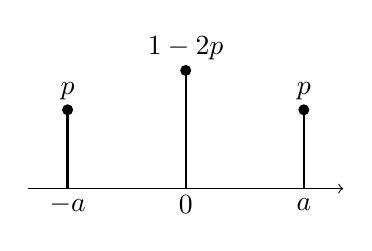
\begin{tikzpicture}[scale=1]
        % Axe horizontal
        \draw[->] (-2,0) -- (2,0);
        % Masses
        \draw[black, thick] (-1.5,0) -- (-1.5,1) node[above, black] {$p$};
        \draw[black, thick] (0,0) -- (0,1.5) node[above, black] {$1 - 2p$};
        \draw[black, thick] (1.5,0) -- (1.5,1) node[above, black] {$p$};
        % Points
        \fill[black] (-1.5,1) circle (2pt);
        \fill[black] (0,1.5) circle (2pt);
        \fill[black] (1.5,1) circle (2pt);
           \node at (-1.5,-0.2) {$-a$};
        \node at (0,-0.2) {$0$};
        \node at (1.5,-0.2) {$a$};
    \end{tikzpicture}
    \caption{Symmetric 3-mass\\ (\autoref{subsec;symmthreepoints}).}
    \label{fig:sym-3-mass}
    \end{subfigure}
    \begin{subfigure}{0.3\textwidth}
    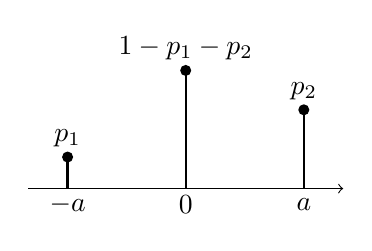
\begin{tikzpicture}[scale=1]
        % Axe horizontal
        \draw[->] (-2,0) -- (2,0);
        % Masses
        \draw[black, thick] (-1.5,0) -- (-1.5,.4) node[above, black] {$p_1$};
        \draw[black, thick] (0,0) -- (0,1.5) node[above, black] {$1-p_1-p_2$};
        \draw[black, thick] (1.5,0) -- (1.5,1) node[above, black] {$p_2$};
        % Points
        \fill[black] (-1.5,.4) circle (2pt);
        \fill[black] (0,1.5) circle (2pt);
        \fill[black] (1.5,1) circle (2pt);
           \node at (-1.5,-0.2) {$-a$};
        \node at (0,-0.2) {$0$};
        \node at (1.5,-0.2) {$a$};
    \end{tikzpicture}

    \caption{Asymmetric 3-mass\\ (\autoref{subsec;asymmthreepoints}).}
    \label{fig:asym-3-mass}
    \end{subfigure}
    \begin{subfigure}{0.3\textwidth}
    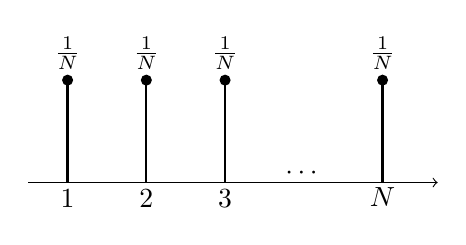
\begin{tikzpicture}[scale=1]
    \def\h{1.3}   % hauteur des tiges
    \def\xN{5}    % position horizontale du bâton "N" (schématique)

    % Axe horizontal
    \draw[->] (0.5,0) -- (\xN+0.7,0);

    % Bâtons pour 1, 2, 3
    \foreach \x/\lab in {1/{$1$}, 2/{$2$}, 3/{$3$}}{
        \draw[black, thick] (\x,0) -- (\x,\h) node[above] {$\frac{1}{N}$};
        \fill[black] (\x,\h) circle (2pt);
        \node at (\x,-0.2) {\lab};
    }

    \pgfmathsetmacro{\dotsx}{\xN-1}
    \node at (\dotsx,0.12) {$\cdots$};

    \draw[black, thick] (\xN,0) -- (\xN,\h) node[above] {$\frac{1}{N}$};
    \fill[black] (\xN,\h) circle (2pt);
    \node at (\xN,-0.18) {$N$};
    \end{tikzpicture}
    \caption{Uniform discrete\\ (\autoref{sec:uniform}).}
    \label{fig:uniform-discrete}
    \end{subfigure}
    \caption{Probability mass function of the discrete distributions covered in the paper.}
    \label{fig:distrib-plots}
\end{figure}


% \begin{figure}[h!]
%     \centering
%     \begin{tikzpicture}[scale=1.2]
%         % Axe horizontal
%         \draw[->] (-2,0) -- (2,0);
%         % Masses
%         \draw[black, thick] (-1,0) -- (-1,0.4) node[above, black] {$p_1$};
%         \draw[black, thick] (0,0) -- (0,1.5) node[above, black] {$1-p_1-p_2$};
%         \draw[black, thick] (1,0) -- (1,1) node[above, black] {$p_2$};
%         % Points
%         \fill[black] (-1,0.4) circle (2pt);
%         \fill[black] (0,1.5) circle (2pt);
%         \fill[black] (1,1) circle (2pt);
%            \node at (-1,-0.2) {$-a$};
%         \node at (0,-0.2) {$0$};
%         \node at (1,-0.2) {$a$};
%     \end{tikzpicture}
%     \caption{Probability mass function of the asymmetric 3-mass distribution.}
%     \label{fig:three_mass_distributionAsym}
% \end{figure}

\section{Characterization of optimal sub-Gaussian variance proxy}\label{sec:charac}

\sloppy{Let $Y$ be some real random variable with finite moments and \( \mu = \mathbb{E}[Y] \). Denote by $M_Y(\lambda):=\ln \left(\mathbb{E}[\exp(\lambda (Y - \mu))]\right)$ the cumulant generating function of the centered random variable $Y-\mu$. In this paper we shall always assume that the random variable $Y$ is such that $M_Y$ is a smooth function}.
Define
\beq g_Y(\lambda;\sigma^2):=\frac{1}{2}\lambda^2\sigma^2- M_Y(\lambda)= \frac{1}{2}\lambda^2\sigma^2-\ln \left(\mathbb{E}[\exp(\lambda (Y - \mu))]\right).\eeq
which is a smooth function of $(\lambda,\sigma^2)$.
We have
\beq g'_Y(\lambda;\sigma^2):= \lambda\sigma^2- M_Y'(\lambda) \, \text{ and } \, g_Y''(\lambda,\sigma^2)=\sigma^2-M_Y''(\lambda).\eeq
Observe that $g_Y(0,\sigma^2)=0=g_Y'(0,\sigma^2)$. Moreover, for $\lambda\neq 0$, the equation $g_Y'(\lambda,\sigma^2)=0$ is equivalent to $\sigma^2=\frac{M_Y'(\lambda)}{\lambda} $. Thus, the system of equations $g_Y(\lambda;\sigma^2)=0$ and $g_Y'(\lambda,\sigma^2)=0$ with $\lambda\neq 0$ is equivalent to  
\beq \sigma^2=\frac{1}{\lambda} M_Y'(\lambda) \text{ and } \lambda\neq 0 \text{ sol. of  } \lambda M_Y'(\lambda)- 2M_Y(\lambda)=0.\eeq

Let us define the set $\mathcal{L}_c^*$ that will play an important role in this paper by
\beq \mathcal{L}_c^*:=\left\{\lambda_c \in \mathbb{R}^* \;\middle|\;  \lambda_c M_Y'(\lambda_c)- 2M_Y(\lambda_c)=0 \,\, \text{ and }\lambda_c \text{ local min. of } g_Y\left(.;\sigma^2=\frac{ M_Y'(\lambda_c)}{\lambda_c}\right) \right\}.\eeq
Then, define the set
\beq \mathcal{S}_c^*=\left\{\frac{M_Y'(\lambda_c)}{\lambda_c}  \;\middle|\; \lambda_c\in \mathcal{L}_c^*\right\}.\eeq
For practical reasons, we complement the two previous sets by defining:
\beq \mathcal{L}_c=\mathcal{L}_c^*\cup\{0\}\,\,, \,\mathcal{S}_c=\mathcal{S}_c^*\cup\{\operatorname{Var}[Y]\}.\eeq 

Let us first make the following observation.
\begin{proposition}[Asymptotics at infinity ans sufficient condition for sub-Gaussianity]\label{AsymptInf}If the cumulant generating function $M_Y$ is a smooth function and satisfy $M_Y(\lambda)\overset{\lambda\to\pm \infty}{=}o(\lambda^2)$ then
\beq \lim_{\lambda\to \pm\infty}g_Y(\lambda;\sigma^2)=+\infty\,,\, \lim_{\lambda\to \pm\infty}g'_Y(\lambda;\sigma^2)=\pm\infty\,,\, \lim_{\lambda\to \pm\infty}g''_Y(\lambda;\sigma^2)=\sigma^2\eeq
and $Y$ is sub-Gaussian. Moreover a sufficient condition is that $Y$ is a bounded random variable.    
\end{proposition}

\begin{proof}The proof is obvious from the definition of $g_Y(\lambda;\sigma^2)=\frac{1}{2}\lambda^2\sigma^2-M_Y(\lambda)$. The sufficient condition is also immediate since if $M$ is a bound for $Y$ then
$|M_Y(\lambda)|\leq \lambda|M+\mu|=o(\lambda^2)$. The fact that $Y$ is sub-Gaussian follows from the fact that there exists $C>0$ such that $|M_Y(\lambda)|\leq C\lambda^2$ for all $\lambda\in \mathbb{R}$. Thus, taking $\frac{C}{2}$ immediately gives that $\sigma^2$ is a variance proxy so that $Y$ is sub-Gaussian.
\end{proof}


Our first main theoretical result is that one can use the sets $\mathcal{S}_c^*$ to characterize the optimal variance proxy.

\begin{theorem}[Characterization of the optimal variance proxy]\label{GeneralCharac} Assume that $M_Y$ is a smooth function and that $M_Y(\lambda)\overset{\lambda\to \pm\infty}{=}o(\lambda^2)$. Then, the optimal variance proxy is characterized by
\beq \sigma_{\mathrm{opt}}^2 = \max\big\{ \operatorname{Var}(Y),\; \sup_{s \in \mathcal{S}_c^*} s \big\}. \eeq   
\end{theorem}

\begin{proof}Let us first mention that \autoref{AsymptInf} implies that the optimal variance proxy is well-defined. Then let us consider $\sigma^2>\max\big\{ \operatorname{Var}(Y),\; \underset{s \in \mathcal{S}_c^*}{\sup} s \big\}$. Since $\sigma^2>\operatorname{Var}[Y]$, we get that $g_Y(.;\sigma^2)$ is locally convex and non-negative around $\lambda=0$.  Let us consider $\lambda_m(\sigma)\neq 0$ a local minimum of $g_Y(.,\sigma^2)$. For simplicity we shall assume that $\lambda_m(\sigma)>0$ but a similar argument is valid if $\lambda_m(\sigma)<0$. Then we have $\partial_{\sigma}[g_Y(\lambda_m(\sigma);\sigma^2)]= g_Y'(\lambda_m(\sigma);\sigma^2) \partial_\sigma \lambda_m(\sigma) + \lambda_m(\sigma)^2\sigma= \lambda_m(\sigma)^2\sigma>0$. Assume by contradiction that $g_Y(\lambda_m(\sigma);\sigma^2)<0$ then increasing $\sigma$ would increase the value of $g_Y(\lambda_m(\sigma);\sigma^2)$. Since $\partial_{\sigma}[g_Y(\lambda_m(\sigma);\sigma^2)]=\lambda_m(\sigma)^2\sigma>0$ there are only two cases: 
\begin{itemize}\item $\lambda_m(\sigma)$ remains outside a positive neighborhood of $0$ denoted $(0,\epsilon)$ when we increase $\sigma$ and thus since $\partial_{\sigma}[g_Y(\lambda_m(\sigma);\sigma^2)]>\epsilon^2 \sigma$ and by assumption $g_Y(\lambda_m(\sigma);\sigma^2)<0$, there exists a value $\sigma_1>\sigma$ for which $g_Y(\lambda_m(\sigma_1);\sigma_1^2)=0$ which is a contradiction because $\sigma_1^2\in \mathcal{S}_c^*$ so that we should have $\sigma\geq \sigma_1$.
\item $\lambda_m(\sigma)\to 0_+$ when we increase $\sigma$. In this case this is a contradiction because $g_Y(.,\sigma^2)$ is locally positive and convex in a positive neighborhood of $0$. Indeed, $g_Y(.,\sigma^2)$ must reach a positive local maximum on $(0,\lambda_m(\sigma))$ that we denote $\lambda_{\text{max}}(\sigma)$. By Rolle's theorem on $(0,\lambda_{\text{max}}(\sigma))$ and $(\lambda_{\text{max}}(\sigma),\lambda_m(\sigma))$, there exist at least two distinct values $(\lambda_1(\sigma),\lambda_2(\sigma))$ with $0<\lambda_1(\sigma)<\lambda_{\text{max}}(\sigma)<\lambda_2(\sigma)<\lambda_m(\sigma)$ such that $g_Y''(\lambda_1(\sigma);\sigma^2)=g_Y''(\lambda_2(\sigma);\sigma^2)=0$. Since $\lambda_m(\sigma)\to 0_+$, we must also have $\lambda_1(\sigma),\lambda_2(\sigma)\to 0_+$ and hence by continuity $g_Y''(0,\sigma^2)\to 0$. But this is impossible since $g_Y''(0;\sigma^2)=(\sigma^2-\operatorname{Var}[Y])>0$ is a positive, increasing function of $\sigma$. 
\end{itemize}
Thus we conclude that for any $\sigma^2>\max\big\{\operatorname{Var}[Y],\underset{s\in \mathcal{S}_c^*}{\sup} s\big\}$, all local minima of $g_Y(.;\sigma^2)$ are non-negative so that since $\underset{\lambda\to \pm \infty}{\lim} g_Y(\lambda;\sigma^2)=+\infty$, $g_Y(.;\sigma^2)$ is non-negative on $\mathbb{R}$. Hence $\sigma^2$ is a variance proxy and thus $\sigma_{\mathrm{opt}}^2\leq \max\big\{\operatorname{Var}[Y],\underset{s\in \mathcal{S}_c^*}{\sup} s\big\}$.

\medskip

\sloppy{Let us prove the converse inequality and assume that $\sigma_{\mathrm{opt}}^2< \max\big\{\operatorname{Var}[Y],\underset{s\in \mathcal{S}_c^*}{\sup} s\big\}$. It is well-known that $\operatorname{Var}[Y]$ is always a lower bound for the optimal variance proxy, thus the last inequality is only possible if  $\operatorname{Var}[Y]<\sigma_{\mathrm{opt}}^2< \underset{s\in \mathcal{S}_c^*}{\sup} s$.} Thus, there exists $s_c\in \mathcal{S}_c^*$ such that $\sigma_{\mathrm{opt}}^2<s_c$, i.e. there exists $\lambda_c\in \mathbb{R}^*$ such that $g_Y(\lambda_c;s_c)=g_Y'(\lambda_c;s_c)=0$ and $\lambda_c$ is a local minimum of $g_Y(.;s_c)$. We have from the fact that the dependence of $g_Y$ relatively to $\sigma$ is quadratic that:
\beq g_Y(\lambda_c,\sigma^2)=g_Y(\lambda_c,s_c) +\frac{1}{2}\lambda_c^2 (\sigma^2-s_c)=\frac{1}{2}\lambda_c^2 (\sigma^2-s_c).\eeq
so that $g_Y(\lambda_c,\sigma^2)<0$ when $\sigma^2<s_c$. This implies that $g_Y(.;\sigma^2)$ is no longer non-negative when $\sigma^2<s_c$ so that $\sigma^2$ is not a variance proxy. This contradicts the fact that $\sigma_{\mathrm{opt}}^2<s_c$ is an optimal variance proxy.
\end{proof}


\begin{remark}The main advantage of the characterization of the optimal variance proxy by \autoref{GeneralCharac} is that it gives a numeric way to obtain the optimal variance proxy in practice. Indeed, in order to determine it, one can numerically solve for the equation $\lambda M_Y'(\lambda)-2M_Y(\lambda)=0$. When numeric solutions are found, one should check numerically if $\lambda$ is a local minimum of $g_Y\left(.;\sigma^2=\frac{M_Y'(\lambda)}{\lambda}\right)$ (a sufficient condition being that $g_Y''\left(\lambda;\sigma^2=\frac{M_Y'(\lambda)}{\lambda}\right)>0$). Collecting all solutions, one picks the optimal variance proxy by looking at the maximal values of $\frac{M_Y'(\lambda)}{\lambda}$ that can easily be computed numerically. In practice, such an algorithm is particularly efficient if the number of solutions of $\lambda M_Y'(\lambda)-2M_Y(\lambda)=0$ is low and if one can bound the intervals on which to look for numeric solutions.  
\end{remark}


\begin{remark}
In practice, for a given family of distributions, one should study the elements of $\mathcal{L}_c^*$. If $\mathcal{L}_c^*$ is non empty, one should compare its elements with the corresponding values of $s_c$ to select the optimal variance proxy. This strategy is particularly efficient when $\mathcal{L}_c^*$ contains very few elements or when these elements can be explicitly expressed in closed-forms.
\end{remark}

The main numerical and theoretical difficulty to study elements of $\mathcal{L}_c^*$ is the fact that they must be local minima of $g_Y(.;\sigma^2)$. This property is tricky to verify because the second derivative may also vanish at this points making the analysis complicated. However, when $g_Y''(.;\sigma^2)$ has very few zeros, it is possible to study its sign and thus remove this complication.  

\begin{proposition}[Positivity when $g_Y''$ has less than one zero on a half-line]\label{Prop01Zeros} Assume that $M_Y$ is a smooth function and that $M_Y(\lambda)\overset{\lambda\to \pm\infty}{=}o(\lambda^2)$. Assume that $g_Y''(.;\sigma^2)$ has no or one zero on $\mathbb{R}_+^*$ for some $\sigma^2\geq \operatorname{Var}[Y]$, then $g_Y(.;\sigma^2)$ is positive on $\mathbb{R}_+^*$. A similar result holds for $\mathbb{R}_-^*$.
\end{proposition}

\begin{proof} The proof is obvious. Indeed, if $g_Y''(.;\sigma^2)$ has no zero on $\mathbb{R}_+^*$, then it is strictly convex on $\mathbb{R}_+^*$ and since $g_Y(0;\sigma^2)=g_Y'(0;\sigma^2)=0$, $g_Y(.;\sigma^2)$ is positive on $\mathbb{R}_+^*$. Similarly, if $g_Y''(.;\sigma^2)$ has a unique zero on $\mathbb{R}_+^*$, then it cannot change sign at this zero, because $g_Y''(0;\sigma^2)=\sigma^2-\operatorname{Var}[Y]\geq 0$ and $\underset{\lambda\to +\infty}{\lim}g_Y''(\lambda;\sigma^2)=\sigma^2>0$. Hence, we conclude similarly that $g_Y(.;\sigma^2)$ is positive on $\mathbb{R}_+^*$. 
\end{proof}

Unfortunately the situation becomes more involved when $g_Y''(.;\sigma^2)$ has more than one zero on a half-line. However, we can still get information when $g_Y''(.;\sigma^2)$ has exactly two zeros on a half-line.

\begin{lemma}[Local minimum when $g_Y''(.;\sigma^2)$ has two positive zeros and $\sigma^2>\text{Var}(Y)$]
\label{LemmaNumber}
%Let us define $\sigma_0^2=\sigma_{\mathrm{opt}}^2 -\frac{1}{2}(\sigma_{\mathrm{opt}}^2-\operatorname{Var}[Y])$ and 
Assume that $M_Y$ is a smooth function and that $M_Y(\lambda)\overset{\lambda\to \pm\infty}{=}o(\lambda^2)$. Moreover, assume that for any $\sigma^2\in \left(\operatorname{Var}[Y],+\infty\right)$, $g_Y''(.;\sigma^2)$ has exactly two positive zeros $(\lambda_1(\sigma),\lambda_2(\sigma))$ such that $0<\lambda_1(\sigma)<\lambda_2(\sigma)$. Then, $g_Y(.;\sigma^2)$ has at most one local minimum  $\lambda_m(\sigma)$ on $\mathbb{R}_+^*$ and it is necessarily located in $\lambda_m(\sigma)\in\left(\lambda_1(\sigma),\lambda_2(\sigma)\right)$. %\textcolor{red}{More precisely, if there exists $\sigma_1^2\in \left(\operatorname{Var}[Y],\sigma_0^2\right)$, where $\sigma_0^2=\sigma_{\mathrm{opt}}^2 -\frac{1}{2}(\sigma_{\mathrm{opt}}^2-\operatorname{Var}[Y])$ such that $g_Y'(.;\sigma_1^2)$ has a zero on $\mathbb{R}_+^*$, then  $g_Y(.;\sigma^2)$ is strictly positive for $\sigma^2\geq\sigma_1^2$ and $g_Y(.;\sigma^2)$ admits a unique local minimum $\lambda_m(\sigma)$ on $\mathbb{R}_+^*$ located in $\lambda_m(\sigma)\in\left(\lambda_1(\sigma),\lambda_2(\sigma)\right)$ for $\operatorname{Var}[Y]<\sigma^2<\sigma_1^2$. Also, $\lambda_m(\sigma)$ is an increasing function of $\sigma$. Olivier: Do we need that in the lemma?}\\ 
Consequently, the equations $g_Y(\lambda,\sigma^2)=0=g_Y'(\lambda,\sigma^2)$ have at most one solution on $\mathbb{R}_+^*\times \left(\operatorname{Var}[Y],+\infty\right)$ and we have that:
\begin{itemize}
    \item if they have no solution, then $g_Y(.;\sigma^2)$ is non-negative on $\mathbb{R}_+$ for any $\sigma^2>\operatorname{Var}[Y]$.
    \item if they have one solution $(\lambda_c,\sigma_c^2)$, then $\lambda_c>0$ is necessarily a local minimum and $g_Y(.;\sigma^2)$ is non-negative on $\mathbb{R}_+$ if and only if $\sigma^2\geq \sigma_c^2$. 
\end{itemize}
A similar result is valid on $\mathbb{R}_-^*$. 
\end{lemma}

\begin{proof}The proof follows from a precise study of variations. Indeed, let us first notice that for any $\sigma^2>\operatorname{Var}[Y]$, we have that $g_Y(.;\sigma^2)$ is locally convex and positive around $\lambda=0$ since $g_Y''(0;\sigma^2)=\sigma^2-\operatorname{Var}[Y]>0$. We also remind that $\underset{\lambda\to \pm \infty}{\lim} g_Y''(\lambda;\sigma^2)=\sigma^2>0$ so that $g_Y(.;\sigma^2)$ is also convex at infinity. Thus, from the assumption that $g_Y''(.;\sigma^2)$ has exactly two zeros $(\lambda_1(\sigma),\lambda_2(\sigma))$ on $\mathbb{R}_+^*$, we conclude that either $g_Y''(.;\sigma^2)$ does not change sign at its zeros and in this case, $g_Y(.;\sigma^2)$ is strictly convex on $\mathbb{R}_+^*$ with $g_Y(0;\sigma^2)=0$ so that it is positive and increasing on $\mathbb{R}_+$, thus there is no solution of $g_Y'(.;\sigma^2)=0$ on $\mathbb{R}_+^*$. Or that $g_Y''(.;\sigma^2)$ is necessarily positive on $(0,\lambda_1(\sigma))$, negative on $(\lambda_1(\sigma),\lambda_2(\sigma))$ and positive on $(\lambda_2(\sigma),+\infty)$. Thus, $g_Y'(.;\sigma^2)$ is increasing on $(0,\lambda_1(\sigma))$ and since $g_Y'(0;\sigma^2)=0$ it is positive on $(0,\lambda_1(\sigma))$. Then, $g_Y'(.;\sigma^2)$ is decreasing on $(\lambda_1(\sigma),\lambda_2(\sigma))$ and then increasing on $(\lambda_2(\sigma),+\infty)$. In particular $g_Y'(.;\sigma^2)$ admits a unique local minimum at $\lambda=\lambda_2(\sigma)$ on $\mathbb{R}_+^*$. Consequently, if $g_Y'(\lambda_2(\sigma);\sigma^2)\geq 0$, then $g_Y(.;\sigma^2)$ is non-negative on $\mathbb{R}_+$ and thus since $g_Y(0;\sigma^2)=0$, we get that $g_Y(.;\sigma^2)$ is non-negative on $\mathbb{R}_+$. Alternatively, if $g_Y'(\lambda_2(\sigma);\sigma^2)<0$, then $g_Y'(.;\sigma^2)$ has exactly two zeros $\lambda_1(\sigma)<\lambda_l(\sigma)<\lambda_r(\sigma)<\lambda_2(\sigma)$ and it is negative on $(\lambda_l(\sigma),\lambda_r(\sigma))$ and positive on $(0,\lambda_l(\sigma))\cup(\lambda_r(\sigma),+\infty)$. Consequently, $g_Y(.;\sigma^2)$ has exactly one local minimum on $\mathbb{R}_+^*$ denoted $\lambda_m(\sigma)$ which is necessarily located in  $(\lambda_1(\sigma),\lambda_2(\sigma))$.
Next, let us observe that:
\beq \partial_\sigma[g_Y'(\lambda_2(\sigma);\sigma^2)]=g_Y''(\lambda_2(\sigma);\sigma^2) \partial_\sigma[\lambda_2(\sigma)]+ 2\sigma\lambda_2(\sigma)=2\sigma\lambda_2(\sigma)>0.\eeq
Thus, the local minimum of $g_Y'(.;\sigma^2)$ is an increasing function of $\sigma$, so that if it is null for a value $\sigma_1$, then it is positive for $\sigma>\sigma_1$ and negative for $\sigma<\sigma_1$.
Finally, let us observe that
\beq  \partial_\sigma[g_Y(\lambda_m(\sigma);\sigma^2)]=g_Y'(\lambda_m(\sigma);\sigma^2) \partial_\sigma[\lambda_m(\sigma)]+ \sigma\lambda_m(\sigma)^2=\sigma\lambda_m(\sigma)^2>0 .\eeq
so that $\lambda_m(\sigma)$ is a increasing function of $\sigma$. Let us denote $(\lambda_c,\sigma_c^2)\in \mathbb{R}_+^*\times \left(\operatorname{Var}[Y],+\infty\right)$ a solution of $g_Y(\lambda,\sigma^2)=0=g_Y'(\lambda,\sigma^2)$, then for $\sigma<\sigma_c$, we have $g_Y(\lambda_m(\sigma);\sigma^2)<0$ while for $\sigma>\sigma_c$, we have $g_Y(\lambda_m(\sigma);\sigma^2)>0$. Since $g_Y(.;\sigma^2)$ has only a unique local minimum $\lambda_m(\sigma)$ and a local maximum on $\mathbb{R}_+^*$ which is always strictly positive, we conclude that we cannot have another solution of $g_Y(\lambda,\sigma^2)=0=g_Y'(\lambda,\sigma^2)$ with $\lambda\in \mathbb{R}_+^*$. When there is no solution, we have $g_Y(\lambda_m(\sigma);\sigma^2)>0$ so that $g_Y(.;\sigma^2)$ is non-negative on $\mathbb{R}_+^*$. When we have a unique solution $(\lambda_c,\sigma_c^2)$, then $g_Y(\lambda_m(\sigma);\sigma^2)>0$ for $\sigma>\sigma_c$, $g_Y(\lambda_m(\sigma_c);\sigma_c^2)=0$ and $g_Y(\lambda_m(\sigma);\sigma^2)<0$ for $\sigma<\sigma_c$ concluding the proof. 
\end{proof}

We complement \autoref{LemmaNumber} with another lemma regarding the situation when $\sigma<\operatorname{Var}(Y)$.

\begin{lemma}[Local minimum when $g_Y''(.;\sigma^2)$ has two positive zeros and $\sigma^2<\operatorname{Var}(Y)$]\label{LemmaNumber2}
Assume that $M_Y$ is a smooth function and that $M_Y(\lambda)\overset{\lambda\to \pm\infty}{=}o(\lambda^2)$ and that for any $\sigma^2\in \left(0,\operatorname{Var}[Y]\right)$, $g_Y''(.;\sigma^2)$ has exactly two zeros $(\lambda_1(\sigma),\lambda_2(\sigma))$ such that $0<\lambda_1(\sigma)<\lambda_2(\sigma)$. Then, there is no solution to the set of equations $g_Y(\lambda;\sigma^2)=0=g_Y'(\lambda;\sigma^2)$ with $\lambda>0$ and $\sigma^2\in \left(0,\operatorname{Var}[Y]\right)$.\\
A similar result holds on $\mathbb{R}_-^*$.
\end{lemma}

\begin{proof}For any $\sigma^2<\operatorname{Var}[Y]$, we have that $g_Y(\lambda\sigma^2)=(\sigma^2-\operatorname{Var}[Y])\lambda^2+o(\lambda^2)$ when $\lambda\to 0_+$. Thus, $g_Y(.;\sigma^2)$ is locally concave and negative around $\lambda=0_+$. Since  $M_Y(\lambda)\overset{\lambda\to \pm\infty}{=}o(\lambda^2)$, we know that $g_Y(.;\sigma^2)$ is locally convex and positive when $\lambda\to +\infty$. Since $g_Y''(.;\sigma^2)$ is assumed to have exactly two positive zeros $\lambda_1(\sigma)<\lambda_2(\sigma)$, we may only have the following cases:
\begin{itemize}
    \item $g''_Y(.;\sigma^2)$ is negative on $(0,\lambda_1(\sigma))$ and changes sign at $\lambda_1(\sigma)$. Thus, it is positive on $(\lambda_1(\sigma),\lambda_2(\sigma))$ and cannot change sign at $\lambda_2(\sigma)$ to remain positive at $+\infty$. Hence, $g''_Y(.;\sigma^2)$ is positive on $(\lambda_1(\sigma),\lambda_2(\sigma))\cup (\lambda_2(\sigma),+\infty)$. Consequently, $g'_Y(.;\sigma^2)$ is decreasing on $(0,\lambda_1(\sigma))$ and increasing on $(\lambda_1(\sigma),+\infty)$. Since $g'_Y(0;\sigma^2)$, we have $g'_Y(\lambda_1(\sigma);\sigma^2)<0$ and since $g'_Y(+\infty;\sigma^2)=+\infty$, $g'_Y$ has only one zero $\lambda_0(\sigma)$ on $\mathbb{R}_+^*$ that satisfies $\lambda_0(\sigma)>\lambda_1(\sigma)$. Moreover, $g'_Y(.;\sigma^2)$ is negative on $(0,\lambda_0(\sigma))$ and positive on $(\lambda_0(\sigma),+\infty)$. Hence, $g_Y(.;\sigma^2)$ is decreasing on $(0,\lambda_0(\sigma))$ and increasing on $(\lambda_1(\sigma),+\infty)$. Since $g_Y(0;\sigma^2)=0$ and $g_Y(+\infty;\sigma^2)=+\infty$, $g_Y$ admits a unique zero $\lambda_*(\sigma)$ on $\mathbb{R}_+^*$ and we have $\lambda_*(\sigma)>\lambda_0(\sigma)$. Hence, there are no simultaneous solutions to $g_Y(\lambda;\sigma^2)=0=g_Y'(\lambda;\sigma^2)$ with $\lambda>0$.
    \item $g''_Y(.;\sigma^2)$ is negative on $(0,\lambda_1(\sigma))$ and does not change sign at $\lambda_1(\sigma)$ so it is negative on $(0,\lambda_2(\sigma))$. In order to be positive at $\lambda\to +\infty$, $g_Y''(.;\sigma^2)$ must change sign at $\lambda=\lambda_2(\sigma)$. Thus, $g_Y'(.;\sigma^2)$ is decreasing on $(0,\lambda_2(\sigma))$ and increasing on $(\lambda_2(\sigma),+\infty)$. Since $g_Y'(0;\sigma^2)=0$ and $g_Y'(+\infty;\sigma^2)=+\infty$, $g_Y'(.;\sigma^2)$ admits a unique zero $\lambda_0(\sigma)$ on $\mathbb{R}_+^*$ and it satisfies $\lambda_0(\sigma)>\lambda_2(\sigma)$. Moreover, $g_Y'(.;\sigma^2)$ is negative on $(0,\lambda_0(\sigma))$ and positive on $(\lambda_0(\sigma),+\infty)$. Since $g_Y(0;\sigma^2)=0$ and $g_Y(+\infty;\sigma^2)=+\infty$, $g_Y(.,\sigma^2)$ is decreasing and negative on $(0,\lambda_0(\sigma))$ and increasing on $(\lambda_0(\sigma),+\infty)$. Hence, $g_Y(.;\sigma^2)$ admits a unique zero $\lambda_*(\sigma)$ on $\mathbb{R}_+^*$ and we have $\lambda_*(\sigma)>\lambda_0(\sigma)$. Hence, there are no simultaneous solutions to $g_Y(\lambda;\sigma^2)=0=g_Y'(\lambda;\sigma^2)$ with $\lambda>0$.
\end{itemize}
\end{proof}

 \autoref{LemmaNumber} and \autoref{LemmaNumber2} can be put together to obtain the following proposition.

\begin{proposition}\label{LemmaMerged}Assume that $M_Y$ is a smooth function and that $M_Y(\lambda)\overset{\lambda\to \pm\infty}{=}o(\lambda^2)$. Moreover assume that for any $\sigma^2>0$, $g_Y''(.;\sigma^2)$ has exactly two zeros $(\lambda_1(\sigma),\lambda_2(\sigma))$ such that $0<\lambda_1(\sigma)<\lambda_2(\sigma)$. Then:
\begin{itemize}
    \item The equations $g_Y(\lambda,\sigma^2)=0=g_Y'(\lambda,\sigma^2)$ have at most one solution on $\mathbb{R}_+^*\times  \mathbb{R}_+^*$. When it exists, this unique solution $(\lambda_0,\sigma_c^2)$ always satisfies $\sigma_c^2>\operatorname{Var}[Y]$.
    \item $g_Y(.;\sigma^2)$ may only become negative on $\mathbb{R}_+$ if and only if the previous set of equations has exactly one solution $(\lambda_0,\sigma_c^2)$  and $\sigma^2< \sigma_c^2$.
\end{itemize}
A similar result holds for $\mathbb{R}_-$.
\end{proposition}

\autoref{Prop01Zeros} and \autoref{LemmaMerged} are interesting to obtain a characterization of the optimal variance proxy when $g_Y''(.;\sigma^2)$ has at most two zeros on each half-lines $\mathbb{R}_\pm^*$. Indeed, in this case the optimal proxy variance is obtained as the maximum of $\operatorname{Var}[Y]$, $\sigma_{c,+}^2$ and $\sigma_{c,-}^2$ where $\sigma_{c,+}^2$ (resp. $\sigma_{c,-}^2$) is the unique solution, when it exists, of the equations $g_Y(\lambda,\sigma^2)=0=g_Y'(\lambda,\sigma^2)$ on $\mathbb{R}_+^*$ (resp. $\mathbb{R}_-^*$). As we shall see, this situation happens for the $3$-mass distributions. It also includes many other standard distributions.

%Another useful result in practice is given in the following general lemma.
%\begin{lemma}[Local minimum when $g_Y''(.;\sigma^2)$ has two positive zeros]
%\label{LemmaMerged}
%Assume that $M_Y$ is a smooth function with $M_Y(\lambda)\overset{\lambda\to \pm\infty}{=}o(\lambda^2)$, and that for any $\sigma^2\in (0,\operatorname{Var}[Y])\cup(\operatorname{Var}[Y],+\infty)$, $g_Y''(.;\sigma^2)$ has exactly two zeros $(\lambda_1(\sigma),\lambda_2(\sigma))$ such that $0<\lambda_1(\sigma)<\lambda_2(\sigma)$. 

%Then the equations $g_Y(\lambda,\sigma^2)=0=g_Y'(\lambda,\sigma^2)$ have at most one solution on $\mathbb{R}_+^*\times((0,\operatorname{Var}[Y])\cup(\operatorname{Var}[Y],+\infty))$. More precisely:

%\begin{enumerate}
%\item \textbf{Case $\sigma^2 < \operatorname{Var}[Y]$:} There is no solution to $g_Y(\lambda,\sigma^2)=0=g_Y'(\lambda,\sigma^2)$ with $\lambda>0$.

%\item \textbf{Case $\sigma^2 > \operatorname{Var}[Y]$:} Let $\sigma_0^2=\sigma_{\mathrm{opt}}^2 -\frac{1}{2}(\sigma_{\mathrm{opt}}^2-\operatorname{Var}[Y])$. 
%\begin{itemize}
 %   \item If there exists $\sigma_1^2\in(\operatorname{Var}[Y],\sigma_0^2)$ such that $g_Y'(.;\sigma_1^2)$ has a zero on $\mathbb{R}_+^*$, then:
%    \begin{itemize}
 %       \item $g_Y(.;\sigma^2)$ is strictly positive for $\sigma^2\geq\sigma_1^2$
%        \item $g_Y(.;\sigma^2)$ admits a unique local minimum $\lambda_m(\sigma)$ on $\mathbb{R}_+^*$ located in $(\lambda_1(\sigma),\lambda_2(\sigma))$ for $\operatorname{Var}[Y]<\sigma^2<\sigma_1^2$
%        \item $\lambda_m(\sigma)$ is an increasing function of $\sigma$
%    \end{itemize}
    
%    \item If the equations $g_Y(\lambda,\sigma^2)=0=g_Y'(\lambda,\sigma^2)$ have:
%    \begin{itemize}
%        \item \textbf{No solution:} then $g_Y(.;\sigma^2)$ is non-negative on $\mathbb{R}_+$ for any $\sigma^2>\operatorname{Var}[Y]$
%        \item \textbf{One solution} $(\lambda_c,\sigma_c^2)$: then necessarily $\lambda_c>0$ is a local minimum, $\sigma_c^2>\operatorname{Var}[Y]$, and $g_Y(.;\sigma^2)$ is non-negative on $\mathbb{R}_+$ if and only if $\sigma^2\geq \sigma_c^2$
%    \end{itemize}
%\end{itemize}
%\end{enumerate}

%A similar result is valid on $\mathbb{R}_-^*$.
%\end{lemma}
%\begin{proof}
%We analyze the two cases separately based on the relationship between $\sigma^2$ and $\operatorname{Var}[Y]$.\\
%\textbf{Case 1}: For any $\sigma^2<\operatorname{Var}[Y]$, we have that $g_Y(\lambda\sigma^2)=(\sigma^2-\operatorname{Var}[Y])\lambda^2+o(\lambda^2)$ when $\lambda\to 0_+$. Thus, $g_Y(.;\sigma^2)$ is locally concave and negative around $\lambda=0_+$. Since  $M_Y(\lambda)\overset{\lambda\to \pm\infty}{=}o(\lambda^2)$, we know that $g_Y(.;\sigma^2)$ is locally convex and positive when $\lambda\to +\infty$. Since $g_Y''(.;\sigma^2)$ is assumed to have exactly two positive zeros $\lambda_1(\sigma)<\lambda_2(\sigma)$, we may only have the following cases:
%\begin{itemize}
%    \item $g''_Y(.;\sigma^2)$ is negative on $(0,\lambda_1(\sigma))$ and changes sign at $\lambda_1(\sigma)$. Thus, it is positive on $(\lambda_1(\sigma),\lambda_2(\sigma))$ and cannot change sign at $\lambda_2(\sigma)$ to remain positive at $+\infty$. Hence, $g''_Y(.;\sigma^2)$ is positive on $(\lambda_1(\sigma),\lambda_2(\sigma))\cup (\lambda_2(\sigma),+\infty)$. Consequently, $g'_Y(.;\sigma^2)$ is decreasing on $(0,\lambda_1(\sigma))$ and increasing on $(\lambda_1(\sigma),+\infty)$. Since $g'_Y(0;\sigma^2)$, we have $g'_Y(\lambda_1(\sigma);\sigma^2)<0$ and since $g'_Y(+\infty;\sigma^2)=+\infty$, $g'_Y$ has only one zero $\lambda_0(\sigma)$ on $\mathbb{R}_+^*$ that satisfies $\lambda_0(\sigma)>\lambda_1(\sigma)$. Moreover, $g'_Y(.;\sigma^2)$ is negative on $(0,\lambda_0(\sigma))$ and positive on $(\lambda_0(\sigma),+\infty)$. Hence, $g_Y(.;\sigma^2)$ is decreasing on $(0,\lambda_0(\sigma))$ and increasing on $(\lambda_1(\sigma),+\infty)$. Since $g_Y(0;\sigma^2)=0$ and $g_Y(+\infty;\sigma^2)=+\infty$, $g_Y$ admits a unique zero $\lambda_*(\sigma)$ on $\mathbb{R}_+^*$ and we have $\lambda_*(\sigma)>\lambda_0(\sigma)$. Hence, there are no simultaneous solutions to $g_Y(\lambda;\sigma^2)=0=g_Y'(\lambda;\sigma^2)$ with $\lambda>0$.
%    \item $g''_Y(.;\sigma^2)$ is negative on $(0,\lambda_1(\sigma))$ and does not change sign at $\lambda_1(\sigma)$ so it is negative on $(0,\lambda_2(\sigma))$. In order to be positive at $\lambda\to +\infty$, $g_Y''(.;\sigma^2)$ must change sign at $\lambda=\lambda_2(\sigma)$. Thus, $g_Y'(.;\sigma^2)$ is decreasing on $(0,\lambda_2(\sigma))$ and increasing on $(\lambda_2(\sigma),+\infty)$. Since $g_Y'(0;\sigma^2)=0$ and $g_Y'(+\infty;\sigma^2)=+\infty$, $g_Y'(.;\sigma^2)$ admits a unique zero $\lambda_0(\sigma)$ on $\mathbb{R}_+^*$ and it satisfies $\lambda_0(\sigma)>\lambda_2(\sigma)$. Moreover, $g_Y'(.;\sigma^2)$ is negative on $(0,\lambda_0(\sigma))$ and positive on $(\lambda_0(\sigma),+\infty)$. Since $g_Y(0;\sigma^2)=0$ and $g_Y(+\infty;\sigma^2)=+\infty$, $g_Y(.,\sigma^2)$ is decreasing and negative on $(0,\lambda_0(\sigma))$ and increasing on $(\lambda_0(\sigma),+\infty)$. Hence, $g_Y(.;\sigma^2)$ admits a unique zero $\lambda_*(\sigma)$ on $\mathbb{R}_+^*$ and we have $\lambda_*(\sigma)>\lambda_0(\sigma)$. Hence, there are no simultaneous solutions to $g_Y(\lambda;\sigma^2)=0=g_Y'(\lambda;\sigma^2)$ with $\lambda>0$.
%\end{itemize}
%\textbf{Case 2}: For $\sigma^2 > \operatorname{Var}[Y]$, the proof follows from a precise study of variations. Indeed, let us first notice that for any $\sigma^2>\operatorname{Var}[Y]$, we have that $g_Y(.;\sigma^2)$ is locally convex and positive around $\lambda=0$ since $g_Y''(0;\sigma^2)=\sigma^2-\operatorname{Var}[Y]>0$. We also remind that $\underset{\lambda\to \pm \infty}{\lim} g_Y''(\lambda;\sigma^2)=\sigma^2>0$ so that $g_Y(.;\sigma^2)$ is also convex at infinity. Thus, from the assumption that $g_Y''(.;\sigma^2)$ has exactly two zeros $(\lambda_1(\sigma),\lambda_2(\sigma))$ on $\mathbb{R}_+^*$, we conclude that either $g_Y''(.;\sigma^2)$ does not change sign at its zeros and in this case, $g_Y(.;\sigma^2)$ is strictly convex on $\mathbb{R}_+^*$ with $g_Y(0;\sigma^2)=0$ so that it is positive and increasing on $\mathbb{R}_+$, thus there is no solution of $g_Y'(.;\sigma^2)=0$ on $\mathbb{R}_+^*$. Or that $g_Y''(.;\sigma^2)$ is necessarily positive on $(0,\lambda_1(\sigma))$, negative on $(\lambda_1(\sigma),\lambda_2(\sigma))$ and positive on $(\lambda_2(\sigma),+\infty)$. Thus, $g_Y'(.;\sigma^2)$ is increasing on $(0,\lambda_1(\sigma))$ and since $g_Y'(0;\sigma^2)=0$ it is positive on $(0,\lambda_1(\sigma))$. Then, $g_Y'(.;\sigma^2)$ is decreasing on $(\lambda_1(\sigma),\lambda_2(\sigma))$ and then increasing on $(\lambda_2(\sigma),+\infty)$. In particular $g_Y'(.;\sigma^2)$ admits a unique local minimum at $\lambda=\lambda_2(\sigma)$ on $\mathbb{R}_+^*$. Consequently, if $g_Y'(\lambda_2(\sigma);\sigma^2)\geq 0$, then $g_Y(.;\sigma^2)$ is non-negative on $\mathbb{R}_+$ and thus since $g_Y(0;\sigma^2)=0$, we get that $g_Y(.;\sigma^2)$ is non-negative on $\mathbb{R}_+$. Alternatively, if $g_Y'(\lambda_2(\sigma);\sigma^2)<0$, then $g_Y'(.;\sigma^2)$ has exactly two zeros $\lambda_1(\sigma)<\lambda_l(\sigma)<\lambda_r(\sigma)<\lambda_2(\sigma)$ and it is negative on $(\lambda_l(\sigma),\lambda_r(\sigma))$ and positive on $(0,\lambda_l(\sigma))\cup(\lambda_r(\sigma),+\infty)$. Consequently, $g_Y(.;\sigma^2)$ has exactly one local minimum on $\mathbb{R}_+^*$ denoted $\lambda_m(\sigma)$ which is necessarily located in  $(\lambda_1(\sigma),\lambda_2(\sigma))$.
%Next, let us observe that:
%\beq \partial_\sigma[g_Y'(\lambda_2(\sigma);\sigma^2)]=g_Y''(\lambda_2(\sigma);\sigma^2) \partial_\sigma[\lambda_2(\sigma)]+ 2\sigma\lambda_2(\sigma)=2\sigma\lambda_2(\sigma)>0\eeq
%Thus, the local minimum of $g_Y'(.;\sigma^2)$ is an increasing function of $\sigma$, so that if it is null for a value $\sigma_1$, then it is positive for $\sigma>\sigma_1$ and negative for $\sigma<\sigma_1$.
%Finally, let us observe that
%\beq  \partial_\sigma[g_Y(\lambda_m(\sigma);\sigma^2)]=g_Y'(\lambda_m(\sigma);\sigma^2) \partial_\sigma[\lambda_m(\sigma)]+ \sigma\lambda_m(\sigma)^2=\sigma\lambda_m(\sigma)^2>0\eeq

%so that $\lambda_m(\sigma)$ is a increasing function of $\sigma$. Let us denote $(\lambda_c,\sigma_c^2)\in \mathbb{R}_+^*\times \left(\operatorname{Var}[Y],+\infty\right)$ a solution of $g_Y(\lambda,\sigma^2)=0=g_Y'(\lambda,\sigma^2)$, then for $\sigma<\sigma_c$, we have $g_Y(\lambda_m(\sigma);\sigma^2)<0$ while for $\sigma>\sigma_c$, we have $g_Y(\lambda_m(\sigma);\sigma^2)>0$. Since $g_Y(.;\sigma^2)$ has only a unique local minimum $\lambda_m(\sigma)$ and a local maximum on $\mathbb{R}_+^*$ which is always strictly positive, we conclude that we cannot have another solution of $g_Y(\lambda,\sigma^2)=0=g_Y'(\lambda,\sigma^2)$ with $\lambda\in \mathbb{R}_+^*$. When there is no solution, we have $g_Y(\lambda_m(\sigma);\sigma^2)>0$ so that $g_Y(.;\sigma^2)$ is non-negative on $\mathbb{R}_+^*$. When we have a unique solution $(\lambda_c,\sigma_c^2)$, then $g_Y(\lambda_m(\sigma);\sigma^2)>0$ for $\sigma>\sigma_c$, $g_Y(\lambda_m(\sigma_c);\sigma_c^2)=0$ and $g_Y(\lambda_m(\sigma);\sigma^2)<0$ for $\sigma<\sigma_c$ concluding the proof.
%\end{proof}





\section{Application to 3-mass distributions}\label{sec:3-mass}



In this section, we undertake a detailed analysis of the sub-Gaussian properties of three-mass discrete distributions supported on $\{-a,0,a\}$. Our objective is to characterize the optimal variance proxy $\sigma^2_{\mathrm{opt}}$ and to delineate the regimes in which strict sub-Gaussianity holds.  

In the \textit{symmetric case}, where the outer masses are equally weighted, we establish two distinct behaviors. When the parameter satisfies $p \geq \tfrac{1}{6}$, the distribution is strictly sub-Gaussian and the optimal variance proxy coincides with the variance,
\[
\sigma^2_{\mathrm{opt}} = \mathrm{Var}[X] = 2p.
\]
In contrast, for $p < \tfrac{1}{6}$, strict sub-Gaussianity fails, and the optimal variance proxy is determined by a critical parameter $\lambda_c > 0$ solving a coupled system of equations.  

In the \textit{asymmetric case}, where the mass probabilities at $-a$ and $a$ are not equal, the situation is more intricate. If the central mass satisfies $p_3 \leq 4\sqrt{p_1p_2}$, then an explicit closed-form expression is available:
\[
\sigma^2_{\mathrm{opt}} = \frac{2(p_2 - p_1)}{\ln\!\left(\tfrac{p_2}{p_1}\right)}.
\]
When $p_3 > 4\sqrt{p_1p_2}$, the characterization of $\sigma^2_{\mathrm{opt}}$ requires the analysis of a nonlinear equation whose solution yields the critical value determining the transition between variance proxies.  
 
%\textcolor{red}{Olivier: Can we put a summary of all important results of the asymmetric case. And a graph summarizing the situation.}
\subsection{Symmetric 3-mass distribution}\label{subsec;symmthreepoints}

Let $X$ be a discrete random variable on the set $\{-a,0,a\}$ where a is a fixed positive real number and
\begin{equation}
    \P(X=-a)=p\,,\, \P(X=0)=1-2p\,,\, \P(X=a)=p
\end{equation}
where $p\in \left( 0,\frac{1}{2}\right)$, see \autoref{fig:sym-3-mass}.
We may define $Y=\frac{1}{a}X$ and use the fact that $\sigma_{\mathrm{opt}}[Y]=\frac{1}{a}\, \sigma_{\mathrm{opt}}[X]$. Thus, we may restrict to $a=1$.\\

In the special case where $p=\frac{1}{2}$ the random variable $X$ reduces to the symmetric Rademacher distribution:
\begin{equation}
    \P(X=-1)= \P(X=1)= \frac{1}{2}.
\end{equation}
This distribution is known to be strictly sub-Gaussian, as shown in \cite{arbel2020strict}.\\
Under these restrictions, we have
\beq \mu:=\E[Y]=0\,\,,\,\, \sigma^2:=\operatorname{Var}[Y]=2p.\eeq
For any $\sigma>0$, we have that $\sigma^2$ is a variance proxy of $Y$ if and only if
\beq \E\left[e^{\lambda (Y-\mu)}\right]=p e^{\lambda }+ pe^{-\lambda } +1-2p\leq e^{\frac{\lambda^2\sigma^2}{2}} \,\, ,\,\, \forall \, \lambda\in \mathbb{R} .\eeq
This inequality is equivalent to
\beq g_{\sigma,p}(\lambda):=\frac{\lambda^2\sigma^2}{2}-\ln( 2p\cosh \lambda +1-2p)\geq 0 \,\,,\,\,  \forall \, \lambda\in \mathbb{R} .\eeq
Since $g_{\sigma,p}$ is an even function of $\lambda$, this is equivalent to 
\beq g_{\sigma,p}(\lambda):=\frac{\lambda^2\sigma^2}{2}-\ln( 2p\cosh \lambda +1-2p)\geq 0 \,\,,\,\,  \forall \, \lambda\in \mathbb{R}_+ .\eeq
The general theory implies that $\operatorname{Var}[Y]=2p$ is a lower bound for the optimal variance proxy. Consequently, we shall only consider $\sigma\geq \sqrt{2p}$ in the following proof.
\medskip

The function $g_{\sigma,p}$ is obviously a smooth function of $(\lambda,\sigma,p)$ and we have
\bea g^{'}_{\sigma,p}(\lambda)&=&\lambda \sigma^2 -\frac{2p\sinh \lambda }{2p\cosh \lambda +1-2p}\cr 
g^{(2)}_{\sigma,p}(\lambda)&=&\sigma^2+\frac{2p\left(2p\cosh \lambda -\cosh \lambda -2p)\right)}{(2p\cosh \lambda +1-2p)^2}\cr
g^{(3)}_{\sigma,p}(\lambda)&=&\frac{2p\sinh \lambda\left(4p^2+4p-1+2p(1-2p)\cosh \lambda\right) }{(2p\cosh \lambda +1-2p)^3}.
\eea
Let us now observe that 
\beq \forall \, \lambda\in \mathbb{R} \,:\,N_{p}(\lambda):=4p^2+4p-1+2p(1-2p)\cosh \lambda \geq 1.\eeq
and $g^{(3)}_{\sigma,p}(0)=0$. Thus, $g^{(3)}_{\sigma,p}$ and $N_{p}$ have the same sign on $\mathbb{R}_+$. Since $N_{p}'(\lambda)=2p(1-2p)\sinh \lambda$, we get that $N_{p}$ is a strictly increasing function on $\mathbb{R}_+$. Since $N_{p}(0)=6p-1$, we get two distinct cases:
\begin{itemize}
    \item $p\geq \frac{1}{6}$: In this case $N_{p}$ is a positive function on $\mathbb{R}_+$ and so is $g^{(3)}_{\sigma,p}$. It follows that $g_{\sigma,p}^{(2)}$ is a strictly increasing function on $\mathbb{R}_+$. Since $g^{(2)}_{\sigma,p}(0)=\sigma^2-2p\geq0$, it we conclude that $g^{(2)}_{\sigma,p}$ is positive  on $\mathbb{R}_+$. Thus $g^{'}_{\sigma,p}$ is a strictly increasing function on $\mathbb{R}_+$. Furthermore, since $g_{\sigma,p}'(0)=0$ we end up with the fact that $g_{\sigma,p}'$ is a positive function on $\mathbb{R}_+$ and therefore $g_{\sigma,p}$ is an increasing function on $\mathbb{R}_+$. Finally, since $g_{\sigma,p}(0)=0$ we conclude that $g_{\sigma,p}$ is positive on $\mathbb{R}_+$ so that $\sigma$ is a variance proxy. This argument is valid for any $\sigma^2\geq \operatorname{Var}[Y]=2p$ so that $\sigma^2_{opt}[Y]=\operatorname{Var}[Y]=2p$, i.e. {$Y$ is strictly sub-Gaussian}.
    \item $p<\frac{1}{6}$: In this case $N_{p}(0)<0$, and $N_{p}$ is increasing on $\mathbb{R}_+$, tending to $+\infty$ when $\lambda\to +\infty$. Thus since $N_{p}$ is a smooth function, there exists a unique $\lambda_0=\arcosh\left(\frac{1-4p-4p^2}{2p(1-2p)}\right)>0$ such that $N_{p}(\lambda_0)=0$. Moreover $N_{p}$ is strictly negative on $(0,\lambda_0)$ and strictly positive on $(\lambda_0,+\infty)$. These properties immediately extend to $g_{\sigma,p}^{(3)}$. Consequently, $g_{\sigma,p}^{(2)}$ is strictly decreasing on $(0,\lambda_0)$ and strictly increasing on $(\lambda_0,+\infty)$. Additionally, we have $g_{\sigma,p}^{(2)}(0)=\sigma^2-2p\geq 0$ and $g_{\sigma,p}^{(2)}(\lambda_0)=\sigma^2-\frac{(1-2p)^2}{4(1-4p)}$ and $g_{\sigma,p}^{(2)}(+\infty)=\sigma^2>0$. Note that if $\sigma^2\geq \frac{(1-2p)^2}{4(1-4p)}$ then $g^{(2)}_{\sigma,p}$ is positive on $\mathbb{R}_+$ and then it is straightforward to prove that $\sigma$ is a variance proxy using the same final steps as the case $p\geq\frac{1}{6}$. Thus, we conclude that $\sigma_{\text{up}}^2(p):=\frac{(1-2p)^2}{4(1-4p)}$ {is an upper bound for the optimal variance proxy of $Y$}. Note also that $\sigma^2=2p$ is no longer a variance proxy because $g^{'}_{\sigma,p}$ would become strictly decreasing on $(0,\lambda_0)$ and thus strictly negative on this interval (because $g^{'}_{\sigma,p}(0)=0$) and so $g_{\sigma,p}$ would be negative on $(0,\lambda_0)$ (again because $g_{\sigma,p}(0)=0)$. This proves that {for $p<\frac{1}{6}$, $Y$ is not strictly sub-Gaussian}. 
\end{itemize}

Let us be more precise in the case $p<\frac{1}{6}$. As mentioned above, we shall now only consider $2p<\sigma^2<\frac{(1-2p)^2}{4(1-4p)}$. The previous analysis implies that there exists a unique pair $(\lambda_1,\lambda_2)$ such that $0<\lambda_1<\lambda_0<\lambda_2$ and $g_{\sigma,p}^{(2)}(\lambda_1)=g_{\sigma,p}^{(2)}(\lambda_2)=0$. Moreover, $g_{\sigma,p}^{(2)}$ is strictly positive on $(0,\lambda_1)\cup(\lambda_2,+\infty)$ and strictly negative on $(\lambda_1,\lambda_2)$. 
Note that we have explicitly:
\bea \lambda_1&:=&\arcosh\left(  \frac{(1-2p)(1-2\sigma^2)-\sqrt{(1-2p)^2-4(1-4p)\sigma^2 } }{4p\sigma^2}\right)\cr
\lambda_2&:=&\arcosh\left(  \frac{(1-2p)(1-2\sigma^2)+\sqrt{(1-2p)^2-4(1-4p)\sigma^2 } }{4p\sigma^2}\right).
\eea
This implies that $g_{\sigma,p}'$ is increasing on $(0,\lambda_1)$, then decreasing on $(\lambda_1,\lambda_2)$ and finally increasing on $(\lambda_2,+\infty)$. Since $g_{\sigma,p}'(0)=0$ and $g_{\sigma,p}'(+\infty)=+\infty$, the sign of $g_{\sigma,p}'$ is determined by the sign of $g_{\sigma,p}'(\lambda_2)$. Note also that a straightforward computation implies that $g_{\sigma,p}'(\lambda_0)=\sigma^2 \lambda_0\sqrt{(1-6p)(1+2p)(1-4p)}>0$. There are only two cases:
\begin{itemize}
\item $g_{\sigma,p}'(\lambda_2)\geq 0$: In this case $g_{\sigma,p}'$ is positive on $\mathbb{R}_+$ so that $g_{\sigma,p}$ is positive on $\mathbb{R}_+$ and thus $\sigma$ is a variance proxy. Thus an upper bound is $\sigma^2_{\text{up}_2}$ that is the unique solution in $\left(2p,\frac{(1-2p)^2}{4(1-4p)}\right)$ of 
\beq \sigma^2_{\text{up2}}=\frac{2p\sinh\lambda_2(\sigma_{\text{up}_2})}{\lambda_2(\sigma_{\text{up}_2}) (1+2p\cosh \lambda_2(\sigma_{\text{up}_2})-2p) },\eeq
where $\lambda_2(x)=\arcosh\left(  \frac{(1-2p)(1-2x^2)+\sqrt{(1-2p)^2-4(1-4p)x^2 } }{4px^2}\right)$.
\item $g_{\sigma,p}'(\lambda_2)<0$: In this case, there exists a unique pair $(\lambda_3,\lambda_4)$ such that $\lambda_0<\lambda_3<\lambda_2<\lambda_4$ and $g_{\sigma,p}'(\lambda_3)=g_{\sigma,p}'(\lambda_4)=0$. Moreover, $g_{\sigma,p}'$ is positive on $(0,\lambda_3)\cup(\lambda_4,+\infty)$ and negative on $(\lambda_3,\lambda_4)$. This implies that $g_{\sigma,p}$ increases on $(0,\lambda_3)$, then decreases on $(\lambda_3,\lambda_4)$ and finally increases on $(\lambda_4,+\infty)$. In particular, since $g_{\sigma,p}(0)=0$ and $g_{\sigma,p}(+\infty)=+\infty$, $g_{\sigma,p}$ has only one local maximum $\lambda_3$ and one local minimum $\lambda_4$ on $(0,+\infty)$. Moreover, these local extremum satisfy $0<\lambda_3<\lambda_0<\lambda_4$ and $g_{\sigma,p}(\lambda_3)>0$. Eventually the sign of $g_{\sigma,p}(\lambda_4)$ determines if $\sigma$ is a variance proxy or not. Since $g_{\sigma,p}(\lambda_4)$ is a smooth function of $\sigma$, the critical case corresponding to $\sigma_{\mathrm{opt}}$ may happen only when $g_{\sigma_{\mathrm{opt}},p}(\lambda_4)=0$. Since we know that this critical case is achieved on $\left(2p,\frac{1-4p+4p^2}{4(1-4p)}\right)$ we conclude with the following statement.
\end{itemize}

\begin{proposition}\label{Propplower16} Let $p\in \left(0,\frac{1}{6}\right)$, then the optimal variance proxy $\sigma_{\mathrm{opt}}^2$ is the unique solution of 
\bea 0&=&g_{\sigma_{\mathrm{opt}},p}(\lambda_c)=\frac{\lambda_c^2\sigma_{\mathrm{opt}}^2}{2}-\ln( 2p\cosh \lambda_c +1-2p)\cr
0&=&g^{'}_{\sigma_{\mathrm{opt}},p}(\lambda_c)=\lambda_c \sigma_{\mathrm{opt}}^2 -\frac{2p\sinh \lambda_c }{2p\cosh \lambda_c +1-2p}
\eea
where $\lambda_c\in (\lambda_0,+\infty)$ is the unique solution in $\lambda_c$, with $\lambda_0=\arcosh\left(\frac{1-4p-4p^2}{2p(1-2p)}\right)>0$. The optimal variance proxy satisfies $2p<\sigma_{\mathrm{opt}}^2<\frac{(1-2p)^2}{4(1-4p)}$.
\end{proposition}

\begin{figure}
\centering
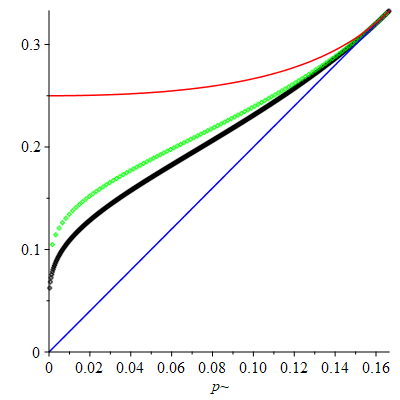
\includegraphics[width=8cm]{NumericPlot.png}
\caption{Numeric plot of the optimal variance proxy (black dots) for $0<p<\frac{1}{6}$. In blue is the variance $2p$ and in red is the upper bound $\sigma_{\text{up}}^2(p):=\frac{(1-2p)^2}{4(1-4p)}$. In green is the numeric evaluation of the upper bound $\sigma_{\text{up2}}^2$.}
\label{241029160152}
\end{figure}

The sub-Gaussian behavior of \(X\) exhibits two distinct regimes as \(p\) varies.
The following theorem summarizes both regimes.

\bigskip

\begin{theorem}[Optimal variance proxy for symmetric three-mass distribution]\label{TheoSymmetric3mass}
Let $X$ be a discrete random variable on the set $\{-a,0,a\}$ where $a > 0$ \text{ and }  $\P(X=-a)=p\,,\, \P(X=0)=1-2p\,,\, \P(X=a)=p$  where $p\in \left( 0,\frac{1}{2}\right)$. Then $X$ is:

\begin{enumerate}
\item[\textbf{(i)}] \emph{Strictly sub-Gaussian regime.}
If \(p \in \left[\tfrac16, \tfrac12\right)\), then \(X\) is strictly sub-Gaussian, i.e.,
\beq \sigma_{\mathrm{opt}}^{2} = \operatorname{Var}(X) = 2p. \eeq

\item[\textbf{(ii)}] \emph{Non-strictly sub-Gaussian regime.}
If \(p \in (0, \tfrac16)\), then \(X\) is not strictly sub-Gaussian. In this case, the optimal variance proxy is given by:
\beq \sigma_{\mathrm{opt}}^{2} = \frac{2p\,\sinh(\lambda_{c})}{\lambda_{c}\,\left(2p\cosh(\lambda_{c}) + 1 - 2p\right)}, \eeq
where \(\lambda_{c} \in (\lambda_{0}, +\infty)\) is the unique solution to \beq p\,\lambda_{c}\,\sinh(\lambda_{c}) - \left(1 - 2p + 2p\cosh(\lambda_{c})\right) \ln\left(1 - 2p + 2p\cosh(\lambda_{c})\right) = 0, \eeq
and \beq \lambda_{0} = \operatorname{arcosh}\left(\frac{1 - 4p - 4p^{2}}{2p(1 - 2p)}\right) > 0. \eeq
\end{enumerate}
\end{theorem}


\subsection{Asymmetric 3-mass distribution}\label{subsec;asymmthreepoints}

Let $X$ be a random variable such that $X(\Omega)=\{-a,0,a\}$ and 
\begin{equation}
    \P(X=-a)=p_1\,,\, \P(X=0)=p_3 = 1-p_1-p_2\,,\, \P(X=a)=p_2.
\end{equation}
where $p_1, p_2, p_3\in \left( 0,1\right)$, see \autoref{fig:asym-3-mass}. Since having one zero weight would correspond to two-mass case,  we will only consider positive weights and $a>0$. We may define $Y=\frac{1}{a}X$ and use the fact that $\sigma_{\mathrm{opt}}[X]=a \sigma_{\mathrm{opt}}[X]$. Thus, we may restrict to $a=1$. We also may assume $p_2 \geq p_1$.  


By considering $Y=-X$ we have
\beq \mu:=\E[Y]=-p_1+p_2 \geq 0\,\,,\,\, \sigma^2:=\operatorname{Var}[Y]=p_1+p_2-(-p_1+p_2)^2 .\eeq
For any $\sigma>0$, we have that $\sigma$ is a variance proxy of $Y$ if and only if
\beq \E\left[e^{\lambda Y}\right]=p_1 e^{-\lambda }+ p_2e^{\lambda } +1-p_1-p_2\leq e^{(\frac{\lambda^2\sigma^2}{2}+\lambda \mu)} \,\, ,\,\, \forall \, \lambda\in \mathbb{R} .\eeq
This inequality is equivalent to
\beq g_{\sigma,p}(\lambda):=\frac{\lambda^2\sigma^2}{2}-\ln(u_{0;p_1, p_2}(\lambda))+\lambda \mu \geq 0 \,\,,\,\,  \forall \, \lambda\in \mathbb{R}.\eeq
With  $u_{0;p_1, p_2}(\lambda) := p_1e^{-\lambda}+p_2e^{\lambda}+1-p_1-p_2$ a smooth function and  $u_{0;p_1, p_2}(\lambda) > 0 \text{ , } \forall \lambda \in \mathbb{R}$. Thus the function $g_{\sigma,p}$ is a smooth function of $(\lambda,\sigma,p)$. For convenience we will use simply $u_0(\lambda)$ and we define
\beq u_{i}(\lambda)=u_{i-1}'(\lambda),   \  i  \in \{1,2,3\} \,\,,\,\,  \forall \, \lambda\in \mathbb{R}.\eeq
We have $u_1(\lambda) = - p_1e^{-\lambda} + p_2e^{\lambda}$ and we observe that $u_2(\lambda) = u_0(\lambda)-p_3$, $u_3(\lambda) = u_1(\lambda)$ and $u_1^2(\lambda)=(u_0(\lambda)-p_3)^2-4p_1p_2$ for all $\lambda \in \mathbb{R}$ \\
%Since $g_{\sigma,p}$ is an even function of $\lambda$, this is equivalent to 
%\beq g_{\sigma,p}(\lambda):=\frac{\lambda^2\sigma^2}{2}-\ln( 2p\cosh \lambda +1-2p)\geq 0 \,\,,\,\,  %\forall \, \lambda\in \mathbb{R}_+\eeq
The general theory implies that $\operatorname{Var}[Y]=p_1+p_2-(-p_1+p_2)^2$ is a lower bound for the optimal variance proxy. In other words, if $\sigma<\sqrt{p_1+p_2-(-p_1+p_2)^2}$ then $\sigma$ is not a variance proxy. Consequently, we shall only consider $\sigma \geq\sqrt{p_1+p_2-(-p_1+p_2)^2}$ in the following proof.
%\medskip

The function $g_{\sigma,p}$ a smooth function of $(\lambda,\sigma,p)$ and its first derivatives can be expressed as:

\bea g^{'}_{\sigma,p}(\lambda)&=&\lambda \sigma^2 -\frac{u_1(\lambda)}{u_0(\lambda)} + \mu \cr 
g^{(2)}_{\sigma,p}(\lambda)&=& \sigma^2-\frac{u_0(\lambda)p_3-p_3^2+4p_1p_2}{u_0(\lambda)^2}\cr
g^{(3)}_{\sigma, p}(\lambda)&=& u_1(\lambda)\frac{p_3u_0(\lambda)+8p_1p_2-2p_3^2}{u_0(\lambda)^3}.
\eea
Note in particular that $g^{(3)}_{\sigma, p}$ does not depend on $\sigma$. Moreover, $g^{(3)}_{\sigma, p}$ can be written as
\beq\label{g3} g^{(3)}_{\sigma, p}(\lambda) = \frac{u_1(\lambda)N_{p_1,p_2}(\lambda)}{u_0(\lambda)^3}. \eeq
where $N_{p_1,p_2}(\lambda) := p_3u_0(\lambda)+8p_1p_2-2p_3^2$. Observe that $u_0(\lambda)$ is strictly positive on $\mathbb{R}$. Therefore, the function $g_{\sigma, p}^{(3)}$ and $u_1 N_{p_1, p_2} $ share the same sign. We know that $u_1$ changes sign at $\lambda_0 := -\frac{1}{2}\ln(\frac{p_2}{p_1})$ assuming that $p_2\geq p_1$ we have $\lambda_0 \leq 0$. Hence, to determine the sign of $g^{(3)}_{\sigma, p}$, it remains to analyze the sign of $N_{p_1, p_2}$. For this purpose, it is sufficient to  study the sign of the polynomial
\bea P(X) :=p_2p_3X^2+(8p_1p_2-p_3^2)X+p_3p_1, \text{where}\  X = e^{\lambda} > 0.\eea 
To determine the sign of $P(X)$, we compute its discriminant:
\bea \Delta = (p_3^2)^2 - 20p_1p_2(p_3)^2 + 64p_1^2p_2^2= (p_3^2-4p_1p_2)(p_3^2-16p_1p_2). \eea 
and it gives two different regimes that we shall study separately. In order to perform the study, we shall prove the following lemma.


\subsubsection{Case $p_3\leq 4\sqrt{p_1p_2}$}
In this case, we shall prove the following theorem.
\begin{theorem}[Explicit value of the optimal variance proxy for $p_3\leq 4\sqrt{p_1p_2}$]\label{TheoRegime1} When $p_3\leq 4\sqrt{p_1p_2}$, the optimal variance proxy is given by
\beq \sigma_{\mathrm{opt}}^2= \frac{2(p_2-p_1)}{\ln \frac{p_2}{p_1}}.\eeq
\end{theorem}

\begin{proof}Let us first observe that $\left(2\lambda_0,\sigma_{\mathrm{opt}}^2\right)=\left(-\ln\frac{p_2}{p_1},\sigma_{\mathrm{opt}}^2\right)$ is a solution $(\lambda,\sigma^2)$ of the system of equations
\beq g_{\sigma,p}(\lambda)=0 \text{ and } g^{'}_{\sigma,p}(\lambda) = 0\eeq
Moreover, the case $p_3\leq 4\sqrt{p_1p_2}$ is equivalent to the fact that $\Delta\leq 0$ or $\Delta>0$ with $P$ admitting two strictly negative roots (the sum of roots ($X_1,X_2)$ is $X_1+X_2 = \frac{p_3^2-8p_1p_2}{p_2p_3} < 0$ and the product of roots $X_1 X_2 = \frac{p_1}{p_2}>0$). Thus, the function $N_{p_1,p_2}$ is strictly positive on $\mathbb{R}$. Consequently, $g^{(3)}_{\sigma,p}$ and $u_1(\lambda)$ share the same sign and hence $g_{\sigma,p}^{(3)}$ is strictly negative on $(-\infty,\lambda_0)$ and strictly positive on $(\lambda_{0}, +\infty)$. Furthermore, since $\lim_{\lambda\to \pm \infty} g^{(2)}_{\sigma, p}(\lambda)=\sigma^2$, it follows that $\lambda_0$ is a global minimum of $g^{(2)}_{\sigma, p}$ with value $g^{(2)}_{\sigma,p}(\lambda_{0})=\sigma^2-\frac{2\sqrt{p_1p_2}}{p_3+2\sqrt{p_1p_2}}$. If $\sigma^2\geq\frac{2\sqrt{p_1p_2}}{p_3+2\sqrt{p_1p_2}}$ , then $g^{(2)}_{\sigma,p}$ is non-negative on $\mathbb{R}$ and so $g'_{\sigma,p}$ is a strictly increasing function. Since $g'_{\sigma,p}(0)=0$, $g'_{\sigma,p}$ is negative on $\mathbb{R}_-$ and positive on $\mathbb{R}_+$ and finally $g_{\sigma,p}$ has a global minimum at $\lambda=0$ which is precisely null so it is positive and $\sigma^2$ is a variance proxy. This gives that $\frac{2\sqrt{p_1p_2}}{p_3+2\sqrt{p_1p_2}}$ is an upper bound for the optimal variance proxy. 

On the contrary, if $\sigma^2<\frac{2\sqrt{p_1p_2}}{p_3+2\sqrt{p_1p_2}}$, then $g^{(2)}_{\sigma, p}$ has two distinct zeros $(\lambda_1(\sigma),\lambda_2(\sigma))$ such that $\lambda_1(\sigma)<\lambda_0<\lambda_2(\sigma)\leq 0$. Moreover, since $g_{\sigma,p}''(.;\sigma^2)$ is positive on $\mathbb{R}_+^*$, we get that $g_{\sigma,p}(.;\sigma^2)$ is always positive on $\mathbb{R}_+^*$ for any $\sigma^2\in \left(\operatorname{Var}[Y],\frac{2\sqrt{p_1p_2}}{p_3+2\sqrt{p_1p_2}} \right) $. Since, we have observed that the equations $g_{\sigma,p}(\lambda,\sigma^2)=0=g_{\sigma,p}'(\lambda,\sigma^2)$ admits $\left(2\lambda_0,\frac{2(p_2-p_1)}{\ln \frac{p_2}{p_1}}\right)\in \mathbb{R}_-^*\times \left(\operatorname{Var}[Y],+\infty\right)$ as solution, application of \autoref{LemmaMerged} on $\mathbb{R}_-^*$ implies that $g_{\sigma,p}(.;\sigma^2)$ is non-negative on $\mathbb{R}_-$ if and only if $\sigma^2\geq \frac{2(p_2-p_1)}{\ln \frac{p_2}{p_1}} $. Thus the optimal variance proxy in this case is $\sigma_{\mathrm{opt}}^2= \frac{2(p_2-p_1)}{\ln \frac{p_2}{p_1}}$ . 

\end{proof}

\autoref{TheoRegime1} implies the following corollary.

\begin{corollary}\label{Strictsub-GaussianityRegime1} For $p_3\leq 4\sqrt{p_1p_2}$, the random variable $Y$ is strictly sub-Gaussian if and only if $p_1=p_2=p$. In this symmetric case, the condition $p_3\leq 4\sqrt{p_1p_2}$ is equivalent to $p\geq \frac{1}{6}$. 
\end{corollary}

\begin{proof}The proof is obvious from the fact that in this case $\sigma_{\mathrm{opt}}^2=\frac{2(p_2-p_1)}{\ln \frac{p_2}{p_1}}\geq \operatorname{Var}[Y]=p_1+p_2-(p_2-p_1)^2$ with equality if and only if $p_1=p_2$.
\end{proof}

\begin{figure}[H]
\centering
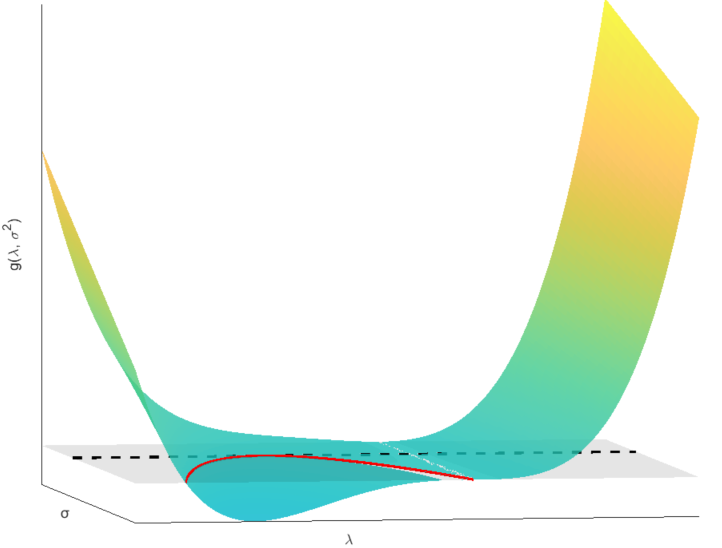
\includegraphics[width=8cm]{g_plot_p1p2-1325.png}
\caption{Numeric plots of $g_{\sigma,p}$ function for fixed $p=(0.13, 0.25)$ varying $\lambda$  and $\sigma^2$ from variance to upper bound $\sigma_{up}$}
\label{241029160153}
\end{figure}

%\textcolor{red}{We should add some plots of the function $g_{\sigma,p}$ for some given values of $(p_1,p_2)$ with varying $\sigma^2$ from the upper bound down to the variance. It is first convex, then now longer convex but with no oscillation and then starts oscillating until it reaches the optimal value. When we hit the variance, it becomes obviously negative locally around $0_-$.}

\subsubsection{Case $p_3>4\sqrt{p_1p_2}$}
In this case, we have $\Delta>0$ and $P$ has two distinct positive roots $0<X_-<X_+$ so that $N_{p_1,p_2}$ has exactly two roots $\lambda_-<\lambda_+$. Their location is given by the following lemma.

\newtheorem*{manuallemma}{Lemma 1.1}
\begin{manuallemma}
\label{lemma:lambda_ordering}
Let $p_1, p_2 \in \mathbb{R}$ such that $p_2 \geq p_1$ and $p_3^2>16p_1p_2$. Then the following inequality holds:
\[
\lambda_0 \leq 0 <\lambda_- <   \lambda_+
\]
\end{manuallemma}
\begin{proof}Let us first observe that we have:
\bea \lambda_{-}= \ln\left(\frac{p_3^2-8p_1p_2 - \sqrt{(p_3^2-4p_1p_2)(p_3^2-16p_1p_2)}}{2p_1p_2}\right) \cr \lambda_{+} =\ln\left(\frac{p_3^2-8p_1p_2 +  \sqrt{(p_3^2-4p_1p_2)(p_3^2-16p_1p_2)}}{2p_1p_2}\right) .\eea
%we have $\sqrt{(p_3^2-4p_1p_2)(p_3^2-16p_1p_2)} > 0$ and $p_3^2-8p_1p_2 > 8p_1p_2$ thus  $p_3^2-8p_1p_2 +  \sqrt{(p_3^2-4p_1p_2)(p_3^2-16p_1p_2)} > 8p_1p_2$ thus $\lambda_+>\ln(4)$ and as $\lambda_0 \leq 0$ we conclude $\lambda_+>\lambda_0$\\
We shall denote for compactness $x := p_3^2>0$, $y := p_1p_2>0$ so that we have the condition $x>16y$. Since $\lambda_0<0$, we only need to prove that $\lambda_->0$. We will now prove that $\lambda_{-} > 0$ under the condition $x > 16y>0$. To establish this result, we proceed through a chain of equivalent inequalities, beginning with the definition of $\lambda_{-}$
\begin{align*}
\lambda_{-} > 0 
&\iff \frac{x - 8y - \sqrt{(x-4y)(x-16y)}}{2y} > 1 \\
&\iff x - 8y - \sqrt{(x-4y)(x-16y)} > 2y \\
&\iff x - 10y > \sqrt{(x-4y)(x-16y)} \\
&\iff (x - 10y)^2 > (x-4y)(x-16y) \quad (\text{because } x > 16y \Rightarrow x-10y > 6y > 0) \\
&\iff x^2 - 20xy + 100y^2 > x^2 - 20xy + 64y^2 \\
&\iff 100y^2 > 64y^2 \\
&\iff 36y^2 > 0 \quad (\text{always valid for  } y \neq 0).
\end{align*}
Thus we get  $\lambda_0 < 0 <\lambda_- <   \lambda_+$ under the condition $p_3^2>16p_1p_2$ ending the proof of the lemma.  
\end{proof}
%\begin{proof}The proof is done by straightforward computations and inequalities and is presented in \autoref{AppendixLemma}.
%\end{proof}

We now analyze the sign of the function  $g_{\sigma, p}(.;\sigma^2)$  separately  on $\mathbb{R}_-^*$ and $\mathbb{R}_+^*$. Let us first observe that the discussion made for $\mathbb{R}_-^*$ in the proof of \autoref{TheoRegime1} is still valid. Thus, $g_{\sigma, p}(.;\sigma^2)$ is non-negative on $\mathbb{R}_-^*$ if and only if $\sigma^2\geq \frac{2(p_2-p_1)}{\ln \frac{p_2}{p_1}}$. Let us now discuss the situation on $\mathbb{R}_+^*$. From \autoref{lemma:lambda_ordering} and \eqref{g3} we get that $g^{(3)}$ is negative on $(-\infty,\lambda_0)\cup\left(\lambda_-(\sigma),\lambda_+(\sigma)\right)$  and positive on $(\lambda_0,\lambda_-(\sigma))\cup\left(\lambda_+(\sigma),+\infty\right)$. Consequently, $g^{(2)}_{\sigma, p}(.;\sigma^2)$ is increasing on $(0,\lambda_-)$ and since $g^{(2)}_{\sigma, p}(0;\sigma^2)=0$ is it thus positive on this interval. Then, $g_{\sigma, p}^{(2)}(.;\sigma^2)$ is decreasing on $(\lambda_-(\sigma),\lambda_+(\sigma))$ and then increasing on $(\lambda_+(\sigma),+\infty)$ with $g_{\sigma, p}^{(2)}(+\infty;\sigma^2)=\sigma^2>0$. Thus, there are only two possible cases: either $g_{\sigma, p}^{(2)}(\lambda_+(\sigma);\sigma^2)\geq 0$ and then $g_{\sigma, p}(.;\sigma^2)$ is strictly convex and positive on $\mathbb{R}_+^*$ or $g^{(2)}_{\sigma, p}(\lambda_+(\sigma);\sigma^2)<0$ in which case $g_{\sigma, p}^{(2)}(.\sigma^2)$ has exactly two zeros $(\lambda_1(\sigma),\lambda_2(\sigma))$ on $\mathbb{R}_+^*$ such that $\lambda_-(\sigma)<\lambda_1(\sigma)<\lambda_+(\sigma)<\lambda_2(\sigma)$. We may thus apply \autoref{LemmaMerged} whose conclusion depends on the existence of a solution $(\lambda,\sigma^2)\in \left(\lambda_-,+\infty\right)*\times \left(\operatorname{Var}[Y],+\infty\right)$ of the equation $g_{\sigma, p}(\lambda;\sigma^2)=0=g_{\sigma, p}'(\lambda;\sigma^2)$. This set of equations is equivalent to
\beq \sigma^2=\frac{1}{\lambda}\left(\frac{u_1(\lambda)}{u_0(\lambda)}-\mu\right)=\frac{1}{\lambda}\left(p_1-p_2+\frac{p_2e^\lambda-p_1e^{-\lambda}}{p_1e^{-\lambda}+p_2e^{\lambda}+1-p_1-p_2}\right),
\eeq
and $\lambda$ positive solution of
\beq \lambda \frac{u_1(\lambda)}{u_0(\lambda)}- 2\ln (u_0(\lambda))+\lambda \mu=0 ,\eeq
i.e.
\beq \label{EqF} F(\lambda):=\lambda u_1(\lambda)-2u_0(\lambda)\ln u_0(\lambda)+ \lambda u_0(\lambda)(p_2-p_1)=0.\eeq
From \autoref{LemmaMerged}, $F(\lambda)=0$ has no solution on $\mathbb{R}_+^*$ such that $\sigma^2=\frac{1}{\lambda}\left(\frac{u_1(\lambda)}{u_0(\lambda)}-\mu\right)<\operatorname{Var}[Y]$. Thus, we have two cases:
\begin{itemize}
    \item If $F$ has a positive zero $\lambda_c>0$ then \autoref{LemmaMerged} implies that this zero is unique on $\mathbb{R}_+^*$ and we get that $\sigma_c^2=\frac{1}{\lambda_c}\left(\frac{u_1(\lambda_c)}{u_0(\lambda_c)}-\mu\right)\geq\operatorname{Var}[Y]$. \autoref{GeneralCharac} implies that the optimal variance proxy is given by
    \beq \sigma_{\mathrm{opt}}^2=\max\left(\frac{2(p_2-p_1)}{\ln \frac{p_2}{p_1}}, \frac{1}{\lambda_c}\left(\frac{u_1(\lambda_c)}{u_0(\lambda_c)}-(p_2-p_1)\right) \right).\eeq
    \item If $F$ has no zero on $\mathbb{R}_+^*$ then $g_{\sigma, p}(.;\sigma^2)$ is positive on $\mathbb{R}_+^*$ and thus the optimal variance proxy is given by $\sigma^2_{\text{opt}}=\frac{2(p_2-p_1)}{\ln \frac{p_2}{p_1}}$.
\end{itemize}

\begin{remark}Note that $\underset{\lambda\to +\infty}{\lim} F(\lambda)=-\infty$ and $F(\lambda)=\frac{1}{6}M_3[Y]\lambda^3+\frac{1}{4}\left(\frac{1}{3}M_4[Y]-\operatorname{Var}[Y]^2\right)\lambda^4+ O(\lambda^5)$, where $M_3[Y]:=\mathbb{E}[(Y-\mu)^3]$ and $M_4[Y]:=\mathbb{E}[(Y-\mu)^4]$. Thus, a sufficient condition for $F$ to admit a positive zero is that $M_3[Y]>0$ or $\left[M_3[Y]=0 \text{ and } \frac{1}{3}M_4[Y]\operatorname{Var}[Y]^2>0\right]$. In particular for $p_1=p_2=p$, we have that $F(\lambda)=\frac{1}{6}p(1-6p)\lambda^4+O(\lambda^5)$ so that for $p>\frac{1}{6}$ (which is the equivalent condition to $p_3>4\sqrt{p_1p_2}$ in this case) $F$ always has a unique positive zero $\lambda_c$ and the corresponding variance $\sigma_c^2=\frac{1}{\lambda_c}\frac{u_1(\lambda_c)}{u_0(\lambda_c)}$ is always greater than $2p=\operatorname{Var}[Y]$ and hence the optimal variance proxy is always $\sigma_{\mathrm{opt}}^2=\sigma_c^2=\frac{1}{\lambda_c}\frac{u_1(\lambda_c)}{u_0(\lambda_c)}$ in the symmetric case $p_1=p_2=p$.
\end{remark}

{\textbf{Outline.}} This paper focuses on three-mass distributions with symmetric support $\{-a, 0, a\}$, in both symmetric and asymmetric cases. To address a more general setting, one may apply translation and dilation to consider a random variable $X$ with support $\{-1, 0, 1+\epsilon\}$, where $\epsilon \in (-1, +\infty)$. This formulation introduces three parameters: $p_1$, $p_2$, and $\epsilon$, which complicate both numerical analysis and exact theoretical treatment. Although an exact analytical characterization appears challenging, identifying necessary and sufficient conditions for strict sub-Gaussianity in this parameterized family remains an open question and a promising direction for future research.ù


% \textcolor{red}{Olivier: There are cases where $F$ does not admit a positive zero. For example $(p_1,p_2)=(0.01, 0.5)$ which belongs to the second regime. }


\section{Application to uniform discrete distributions}\label{sec:uniform}
Let \( X \) be a random variable with finite support defined as \(X(\Omega)=\{x_1, x_2, \ldots, x_N\}\), where $N>1$, and each point is equiprobable: 
\[
  \mathbb{P}(X = x_k) = \frac{1}{N}, \quad \text{for all } k \in \{1,2,\dots,N\}.
\]
We consider that the support points are regularly spaced, such that there exist parameters \( a \in \mathbb{R} \) and  \( h \in  \mathbb{R}^{*}_{+} \) satisfying
 \[
 x_k = ka  + h , \quad \ \forall\, k  \in\ \{1,2,\dots,N\}.
 \]
Introducing the normalized random variable
 \[
 Y = \frac{X-h}{a}.
 \]
and employing the linearity property of the optimal variance proxy, we have the relation
\[
\sigma_{\mathrm{opt}}[X] = a\,\sigma_{\mathrm{opt}}[Y].
\]
Thus, without loss of generality, we can restrict our attention to the simplified case $a=1$ and $h=0$. Under this assumption, the variable $Y$ is uniformly distributed on the integer set $\{1, 2, \ldots, N\}$, see \autoref{fig:uniform-discrete}, with the well-known moments:
\beq
  \mu:=\E[Y]=\frac{N+1}{2}, \quad  \sigma^2:=\operatorname{Var}[Y]=\frac{N^2-1}{12}, \quad \operatorname{\kappa_3}[Y] := \E[(Y-\E[Y])^3]=0.
\eeq
By definition, a real number $\sigma>0$ is said to be a \emph{variance proxy} of $Y$  if and only if it satisfies the following exponential inequality for all $\lambda \in \mathbb{R}$:
\beq
\E\left[e^{\lambda Y}\right]=  \frac{1}{N}\sum_{k=1}^{N} e^{\lambda k} \leq e^{\left(\frac{\lambda^2\sigma^2}{2}+\lambda \mu\right)} \,\, ,\,\, \forall \, \lambda\in \mathbb{R}.
\eeq
This condition can be equivalently rewritten as the non-negativity requirement on the function:
\beq
g_{\sigma,N}(\lambda):=\frac{\lambda^2\sigma^2}{2}-u(\lambda)+\lambda \frac{N+1}{2} \geq 0 \,\,,\,\,  \forall \, \lambda\in \mathbb{R}.
\eeq
Where we define the log-partition function as:
\[
u(\lambda) := \ln\left(\frac{1}{N}\sum_{k=1}^{N} e^{\lambda k}\right).
\]
By general theory, it follows that the variance $\operatorname{Var}[Y]=\frac{N^2-1}{12}$ provides a lower bound for the optimal variance proxy. Hence, in our analysis we consider $\sigma\geq \sqrt{\frac{N^2-1}{12}}$.\\

To characterize the optimal variance proxy, it is essential to study the properties of the function $g_{\sigma, N}$. Observe that $g_{\sigma, N}$ is a smooth function of $(\sigma, \lambda, N)$. Its first three derivatives with respect to $\lambda$ are explicitly computed as:
\begin{align*}
g'_{\sigma,N}(\lambda)   &= \lambda \sigma^2 - u'(\lambda) + \mu \\
g^{(2)}_{\sigma,N}(\lambda) &= \sigma^2 - u^{(2)}(\lambda)\\
g^{(3)}_{\sigma,N}(\lambda) &= - u^{(3)}(\lambda).
\end{align*}
To analyze the properties of the function \( u(\lambda) \), and consequently those of \( g_{\sigma,N}(\lambda) \), we introduce an auxiliary family of probability distributions. This approach allows us to leverage probabilistic tools to study the behavior of \( u(\lambda) \) and its derivatives.\\
%Let \( \mathcal{I} = \{1, \ldots, N\} \). 
For every real number \( \lambda \), consider the family of probability distributions \( (P_\lambda)_{\lambda \in \mathbb{R}} \) on \( \mathcal{I} \) defined by
\beq
P_\lambda(k) = \frac{e^{\lambda k}}{\underset{j=1}{\overset{N}{\sum}}e^{\lambda j}}, \quad \forall \, k\in \{1,\dots,N\}.
\eeq
We denote by \( \mathbb{E}_\lambda[\cdot] \), \( \operatorname{Var}_\lambda[\cdot] \), and \( \operatorname{\kappa}_{3,\lambda[}\cdot] \) the expectation, variance and  third central moment with respect to \( P_\lambda \), respectively. Note that when \( \lambda = 0 \), this distribution reduces to the uniform distribution over \( \mathcal{I} \).
This family of distributions satisfies several fundamental identities, including symmetry properties and a moment derivative formula.
\paragraph{Symmetry identities.}
    \begin{itemize}
        \item \( P_{-\lambda}(k) = P_\lambda(N - k + 1) \),
        \item \( \mathbb{E}_{-\lambda}[Z] = N + 1 - \mathbb{E}_\lambda[Z] \),
        \item \( \operatorname{Var}_{-\lambda}[Z] = \operatorname{Var}_\lambda[Z] \).
    \end{itemize}
\paragraph{Moment derivative identity.} For all integers \( m \geq 1 \),
    \[
    \frac{d}{d\lambda} \mathbb{E}_\lambda[Z^m] = \mathbb{E}_\lambda[Z^{m+1}] - \mathbb{E}_\lambda[Z]\,\mathbb{E}_\lambda[Z^m].
    \]
These identities will be used repeatedly in the analysis of the log-partition function and its derivatives.
\begin{lemma}[Derivatives of log-partition function as moments]\label{lem:log_partition_moments}
The derivatives of \( u(\lambda) \) give the moments of the associated exponential family distribution:
\beq
u'(\lambda) = \mathbb{E}_{\lambda}[Z], \quad u^{(2)}(\lambda) = \operatorname{Var}_{\lambda}[Z], \quad u^{(3)}(\lambda) = \mathbb{E}_{\lambda}[(Z - \mathbb{E}_{\lambda}[Z])^3] = \operatorname{\kappa}_{3,\lambda}[Z].
\eeq
\end{lemma}

\begin{proof}
These identities follow directly from the moment derivative formula combined with the expressions for the first moments. Applying the derivative identity recursively yields the expressions for \( u'(\lambda) \), \( u^{(2)}(\lambda) \), and \( u^{(3)}(\lambda) \), which correspond to the mean, variance, and third centered moment under \( P_\lambda \).
\end{proof}

From Symmetry identities, we know that  $\operatorname{Var}_{\lambda}[X]$ is an even function of $\lambda$. This symmetry allows us to restrict our analysis to $\mathbb{R}_+$. Given the derivative relationship 
 \beq \operatorname{\kappa}_{3,\lambda}[Z] = \frac{d}{d\lambda}\operatorname{Var}_{\lambda}[Z]. \eeq
along with the evenness of the variance, it follows that the the third central moment is an odd function of $\lambda$. Thus we can restrict our analysis to \( \mathbb{R}_+ \).

\begin{lemma}
[Negativity of the third derivative of the log-partition function]\label{lemma:neg_third_deriv}
Let \( N \geq 2 \) be an integer and let \( \lambda > 0 \) be a real number. Then the third derivative of the log-partition function is strictly negative. In other words,
\beq
u^{(3)}(\lambda) = -\frac{N^3 e^{\lambda N}(1 + e^{\lambda N})}{(1 - e^{\lambda N})^3} + \frac{e^{\lambda}(1 + e^{\lambda})}{(1 - e^{\lambda})^3} < 0, \quad \forall\, \lambda\in \mathbb{R^*_+}.
\eeq
Consequently,
\beq
\operatorname{\kappa}_{3,\lambda}[Z] < 0 \text{ for all } \lambda \in \mathbb{R}_+ *.
\eeq
\end{lemma}
\begin{proof}
The explicit expression  of \( u^{(3)}\) follow by direct differentiation of \( u(\lambda) = \ln S(\lambda) \), where $ S(\lambda) = \frac{1}{N}\underset{k=1}{\overset{N}{\sum}}e^{\lambda k}$ and using the closed-form expression for the geometric sum.\\
Consider the auxiliary function
\[
f(t) = \frac{t(t + 1)}{(1 - t)^3}, \quad \text{for } t = e^{\lambda} > 1.
\]
We compute its derivative:
\[
f'(t) = \frac{1 + 4t + t^2}{(1 - t)^4}.
\]
Since both the numerator and the denominator are strictly positive for all \( t > 1 \), we conclude that \( f'(t) > 0 \). Hence, \( f \) is strictly increasing on the interval \( (1, \infty) \).

Now fix \( \lambda > 0 \), so that \( t = e^{\lambda} > 1 \). Since \( N \geq 2 \), we have \( t^N > t \). By the monotonicity of \( f \), it follows that
\[
f(t^N) > f(t),
\]
which yields the inequality
\[
\frac{e^{\lambda N}(1 + e^{\lambda N})}{(1 - e^{\lambda N})^3} > \frac{e^{\lambda}(1 + e^{\lambda})}{(1 - e^{\lambda})^3}.
\]

Furthermore, since \( N^3 \geq 8 \) for all \( N \geq 2 \), we obtain
\[
\frac{N^3 e^{\lambda N}(1 + e^{\lambda N})}{(1 - e^{\lambda N})^3} > \frac{e^{\lambda}(1 + e^{\lambda})}{(1 - e^{\lambda})^3}.
\]

Therefore, the third derivative of the log-partition function satisfies
\[
u^{(3)}(\lambda) 
= - \frac{N^3 e^{\lambda N}(1 + e^{\lambda N})}{(1 - e^{\lambda N})^3}
+ \frac{e^{\lambda}(1 + e^{\lambda})}{(1 - e^{\lambda})^3}
< 0.
\]
which completes the proof.
\end{proof}

\paragraph{Variance proxy optimality.}
\autoref{lemma:neg_third_deriv} shows that
\[
\kappa_{3,\lambda}[Z] = \frac{d}{d\lambda}\operatorname{Var}_{\lambda}[Z] < 0, \quad \forall \lambda > 0.
\]
As \( \operatorname{Var}_{\lambda}[Z] \) is an even function of \( \lambda \), it follows that it is strictly increasing on \( \mathbb{R}_- \), strictly decreasing on \( \mathbb{R}_+ \), and attains a unique global maximum at \( \lambda = 0 \). In particular,
\[
\operatorname{Var}_{\lambda}[Z] \leq \operatorname{Var}_0[Z] = \operatorname{Var}[Y], \quad \forall \lambda \in \mathbb{R}.
\]
    Hence, for any \( \sigma^2 \geq \operatorname{Var}[Z] \), we have \( g_{\sigma,N}^{(2)}(\lambda) = \sigma^2 - \operatorname{Var}_\lambda[Z] \geq 0 \), with equality if and only if \( \lambda = 0 \). Given that \( g_{\sigma,N}^{(2)}(\lambda)\) has no solution on $\mathbb{R^*_+} \text{ or } \mathbb{R^*_-}$, it follows from \autoref{Prop01Zeros} that $g_{\sigma,N}$ is non-negative on $\mathbb{R} $. In addition the system of equations
\[
g_{\sigma,N}(\lambda,\sigma^2) = 0, \quad \frac{\partial}{\partial \lambda} g_{\sigma,N}(\lambda,\sigma^2) = 0 .
\]
admits a unique solution at \( \lambda = 0 \), thus \( Y \) is strictly sub-Gaussian and \beq 
\sigma^2_{\mathrm{opt}}[Y] = \operatorname{Var}[Y] = \frac{N^2 - 1}{12}. \eeq Thus \(X\) is strictly sub-Gaussian and its optimal proxy variance has the form \beq \sigma^2_{\mathrm{opt}}[X] = a^2 \frac{N^2 - 1}{12}. \eeq


\section{Software implementation}\label{sec:software}

To support reproducibility and facilitate the use of state-of-the-art and our theoretical results, 
we developed a Python package to compute the optimal sub-Gaussian variance proxy for a wide range of probability distributions. 
The package handles both discrete and continuous distributions, including truncated Gaussian and Exponential laws. 
It returns whether a given distribution is strictly sub-Gaussian as well as the associated optimal variance proxy. 

The implementation follows a unified principle. 
Whenever a closed-form expression is available, it is returned directly, e.g., Bernoulli, Binomial, Uniform, Discrete Uniform, and certain symmetric laws such as Beta, Kumaraswamy, Triangular, or  three-mass distributions (under specific conditions). 
In contrast, when no closed form exists, the computations relies on the general characterization via
\[
h(\lambda) \;=\; \frac{2}{\lambda^{2}} \, \ln \mathbb{E}\!\left[e^{\lambda(X-\mu)}\right],
\qquad 
\sigma^2_{\text{opt}} \;=\; \sup_{\lambda \in \mathbb{R}} h(\lambda),
\]
where $\mu$ is the mean of the distribution. 
The maximizer of $h(\lambda)$ is located numerically using adaptive grid search combined with robust root-finding algorithms (Brent or bisection). 

For some families, such as the Triangular distribution, the alternative $\Delta$-function formulation recommended in \cite{arbel2020strict} is employed: 
\[
\Delta(\sigma^{2}, \lambda) \;=\; \exp\!\left(\tfrac{1}{2}\lambda^{2}\sigma^{2}\right) \;-\; \mathbb{E}\!\left[e^{\lambda(X-\mu)}\right],
\]
where the optimal variance proxy is the smallest $\sigma^{2}$ such that $\Delta(\sigma^{2}, \lambda) \geq 0$ for all $\lambda$, with equality and stationarity at some $\lambda_0 \in \mathbb{R}$:
\[
\Delta(\sigma_{\mathrm{opt}}^{2}, \lambda_0) = 0, 
\qquad 
\frac{\partial}{\partial \lambda}\Delta(\sigma_{\mathrm{opt}}^{2}, \lambda_0) = 0.
\]

For stability near singular regimes, local Taylor expansions of the cumulant generating function are also employed to represent $\Delta$.\\

In addition, the package also implements the characterization of the optimal variance proxy based on the function 
\[
g_Y(\lambda;\sigma^2)=\tfrac{1}{2}\lambda^2\sigma^2 - M_Y(\lambda),
\]
where $M_Y$ is the cumulant generating function of $Y-\mu$. 
This approach reduces the computation of $\sigma^2_{\mathrm{opt}}$ to solving the coupled system 
\[
g_Y(\lambda;\sigma^2)=0, \qquad g'_Y(\lambda;\sigma^2)=0,
\]
leading to the critical sets $\mathcal{L}_c$ and $\mathcal{S}_c$ introduced in \autoref{sec:charac}. 
This formulation is particularly useful for discrete distributions with a few number of points, such as the three-mass distribution, where it provides a tractable and efficient criterion for identifying candidate values of the variance proxy.\\
To this end, the software integrates efficient bracketing, adaptive grid search, and Brent-type root-finding to implement characterizations above.
This hybrid approach allows the package to combine exact formulas with adaptive numerical optimization, thereby covering both tractable and analytically intractable distributions within a consistent computational framework. 
In addition, the package offers utilities for visualization (plots of $h(\lambda)$, comparisons of $\mathrm{Var}(X)$ vs.\ $\sigma^2_{\text{opt}}$) and supports batch analysis across multiple parameter settings. 
The software provides a comprehensive and user-friendly environment for exploring sub-Gaussian properties, and serves as a computational companion for researchers applying concentration bounds in Bayesian inference, variational methods, and beyond.\\
%GUI description, plots (h(.), and tails), cursors (zoom in/out, range ...), S  
%\section{Future research directions}
\section*{Acknowledgment}
\sloppy{Olivier Marchal was supported by the fundamental junior IUF grant G752IUFMAR, and Julyan Arbel by grant ANR-21-JSTM-0001.}

\newpage
%\section{Software Implementation}\label{sec:software}
%To support reproducibility and facilitate the use of state-of-the-art and our theoretical  results, 
%we developed a python package to compute the optimal sub-Gaussian variance proxy for a wide range of probability distributions. 
%The package handles both discrete and continuous distributions, including some truncated distributions as Gaussian and exponential. The package returns whether a given distribution is strictly sub-Gaussian as well as the associated optimal variance proxy. 
%The implementation follows a unified principle: whenever a closed-form expression of the variance proxy is available, it is returned directly (e.g., Bernoulli, Binomial, Uniform, Discrete Uniform, and certain symmetric laws such as Beta, Kumaraswamy, Triangular, or symmetric three-mass distributions under specific conditions). 

%In contrast, when no closed form exists, in the general case, the computation relies on the characterization by the function
%\[
%h(\lambda) \;=\; \frac{2}{\lambda^{2}} \, \ln \mathbb{E}\!\left[e^{\lambda(X-\mu)}\right],
%\]
%where $\mu$ is the mean of the distribution. 
%The optimal variance proxy is then given by
%\[
%\sigma^2_{\text{opt}} \;=\; \sup_{\lambda \in \mathbb{R}} h(\lambda),
%\]
%and is obtained numerically by locating the maximizer of $h(\lambda)$ through adaptive grid search and Brent or bisection root-finding methods. 
%In specific situations (eg Triangular distribution) another characterization using  $\Delta$-function  as recommended in \cite{arbel2020strict}. The $\Delta$-function is defined by:
%\[
%\Delta(\sigma^{2}, \lambda) \;=\; \exp\!\left(\tfrac{1}{2}\lambda^{2}\sigma^{2}\right) \;-\; \mathbb{E}\!\left[e^{\lambda(X-\mu)}\right],
%\]
%here $\lambda \in \mathbb{R}$ and $\mu$ is the mean of the distribution. 
%The optimal variance proxy is then identified as the smallest $\sigma^{2}$ such that $\Delta(\sigma^{2}, \lambda) \geq 0$ for all $\lambda$, and there exist $\lambda_0 \in \mathbb{R}$ such that: 
%\[
%\frac{\partial}{\partial \lambda}\Delta(\sigma_{\mathrm{opt}}^{2}, \lambda_0) = 0 \quad \text{and} \quad \Delta(\sigma_{\mathrm{opt}}^{2}, \lambda_0) = 0
%\]
%To this end, the software integrates efficient bracketing, adaptive grid search, and Brent-type root-finding to solve the system of equation above.
%to test feasibility of a candidate variance. 
%For stability near singular regimes, local Taylor expansions of the cumulant generating function are employed. 
%This hybrid approach allows the software to combine exact formulas when available with reliable adaptive methods otherwise, thereby covering both tractable and analytically intractable distributions within a consistent computational framework. 
%In addition, the package offers utilities for visualization (plots of $h(\lambda)$, comparisons of $\mathrm{Var}(X)$ vs.\ $\sigma^2_{\text{opt}}$) and supports batch analysis across multiple parameter settings. 
%Overall, this software provides a comprehensive and user-friendly environment for exploring sub-Gaussian properties, and serves as a computational companion for researchers applying concentration bounds in Bayesian inference, variational methods, and beyond.






\newpage


% \newpage
% \section*{Technical Results}

% \paragraph{Acknowledgment.}
% % ----------------------------------------------------------------
% We would like to thank ...
\bibliographystyle{plainnat}
\bibliography{references}


\appendix
\end{document}